\documentclass{article}

% arxiv-standard packages
\usepackage[preprint]{neurips_2024}   % swap to [final] for camera-ready
% Override the default "Preprint. Under review." footer for arXiv submission
\makeatletter
\renewcommand{\@noticestring}{Preprint. arXiv submission.}
\makeatother
\widowpenalty=10000
\clubpenalty=10000
\usepackage[utf8]{inputenc}
\usepackage[T1]{fontenc}
\usepackage{hyperref}
\usepackage{url}
\usepackage{booktabs}
\usepackage{amsfonts}
\usepackage{amsmath}
\usepackage{amssymb}
\usepackage{nicefrac}
\usepackage{microtype}
\usepackage{xcolor}
\usepackage{graphicx}
\usepackage{multirow}
\usepackage{amsthm}
\usepackage{listings}
\lstset{%
  basicstyle=\ttfamily\small,
  language={},
  frame=single,
  framerule=0.4pt,
  backgroundcolor=\color{gray!10},
  xleftmargin=10pt,
  xrightmargin=10pt,
  aboveskip=6pt,
  belowskip=4pt,
  breaklines=false,
  columns=fixed,
}

\newtheorem{proposition}{Proposition}
\newtheorem{corollary}{Corollary}
\newtheorem{definition}{Definition}

\title{Dynamic Attentional Context Scoping:\\
Agent-Triggered Focus Sessions for\\
Isolated Per-Agent Steering in Multi-Agent LLM Orchestration}

\author{%
  Nickson Patel \\
  Independent Researcher \\
  \texttt{nicksonpatel@gmail.com}
}

\begin{document}
\maketitle
\renewcommand{\arraystretch}{1.15}

%-----------------------------------------------------------------------
\begin{abstract}
Multi-agent LLM orchestration systems suffer from \emph{context pollution}:
when $N$ concurrent agents share an orchestrator's context window,
cross-agent interference degrades steering quality systematically.
We formalise this as the \textbf{Multi-Agent Attention Allocation Problem
(MAAAP)}: given a token budget $T$ and $N$ agents each requiring focused
steering, allocate context to maximise total decision quality.
We introduce the \textbf{Context Interference Principle (CIP)},
which predicts that flat-context error grows as $O(N)$ due to
cross-agent interference while isolation-based policies maintain
near-constant error.
We propose \textbf{Dynamic Attentional Context Scoping (DACS)}, a
mechanism in which the orchestrator dynamically switches between a
lightweight \textsc{Registry} mode (compact per-agent summaries) and
an agent-triggered \textsc{Focus} mode (full context of the requesting
agent only).
DACS operates as a deterministic hard-attention policy over agents:
at each steering event, exactly one agent receives full fidelity while
all others are compressed to registry entries.
We evaluate across 240 controlled trials plus external benchmark
validation in five experimental phases:
$N$-scaling ($N{\in}\{3,5,10\}$), agent diversity, decision density
($D$ up to 15), real-agent validation (Claude Haiku~4.5), and
GAIA Level-1 factual Q\&A~\citep{gaia2023} ($N{=}3$, exact-match scoring).
DACS achieves $90.0$--$98.4\%$ steering accuracy versus $21.0$--$60.0\%$
for a flat-context baseline ($p < 0.0001$ throughout).
Power-law fits on five data points ($N\in\{3,5,10,15,20\}$) confirm CIP:
baseline error scales as
$\varepsilon \propto N^{0.19}$ ($R^2 = 0.69$) while DACS error remains
near-constant ($<10\%$ at all $N$).
Ablation studies confirm that focus isolation is both necessary and
sufficient: removing registry context has negligible impact ($p > 0.67$),
while removing isolation collapses accuracy to baseline levels.
Phase~5 (GAIA Level-1) confirms the no-harm property:
DACS matches baseline exact-match accuracy ($86.8\%$ vs.\ $87.5\%$,
$p{=}0.79$) while retaining $1.47\times$ context efficiency.
All code and data are released at
\href{https://github.com/nicksonpatel/dacs-agent-focus-mode}{\texttt{github.com/nicksonpatel/dacs-agent-focus-mode}}.
\end{abstract}

%-----------------------------------------------------------------------
\section{Introduction}
\label{sec:intro}

Attention is a scarce resource in multi-agent LLM systems.
When a single orchestrator manages $N$ concurrent agents, each agent's
task context---partial outputs, domain-specific state, pending
decisions---competes for space in the orchestrator's context window.
This competition is not merely a capacity problem:
it introduces systematic \emph{cross-agent interference} that degrades
the quality of every steering decision.
We call this \emph{context pollution},
and we show it is the dominant failure mode in multi-agent orchestration,
not model capability, not architecture topology, not memory compression.

\paragraph{The problem at scale.}
Consider an orchestrator managing three agents: a code writer implementing
a BST, a researcher surveying transformer attention, and a data processor
handling CSV encoding.
When the code writer asks ``should I use recursive or iterative
traversal?'', the orchestrator's context simultaneously holds the
researcher's attention mechanism analysis and the data processor's UTF-8
encoding problem.
Empirically, flat-context accuracy collapses from 60\% at $N{=}3$ to
21\% at $N{=}10$ and degrades further as agents accumulate longer
decision histories.

\paragraph{From observation to theory.}
We formalise this failure mode as the \textbf{Multi-Agent Attention
Allocation Problem (MAAAP)}: given a token budget $T$ and $N$ agents
each requiring independent steering decisions of quality $Q_i$, how
should the orchestrator allocate its context window to
maximise $\sum_i Q_i$?
We introduce the \textbf{Context Interference Principle (CIP)},
which decomposes decision quality as
$Q_i = S_i - \lambda \sum_{j \neq i} I(C_j, F_i)$,
where $S_i$ is the signal from agent $i$'s relevant context,
$I(C_j, F_i)$ measures interference from agent $j$'s context on
agent $i$'s decision, and $\lambda$ is an interference coefficient.
CIP predicts that flat-context error grows linearly with $N$
(each additional agent contributes $\lambda \bar{I}$ interference),
while an isolation policy that limits $C_j$ to compact summaries
$r_j$ maintains near-constant error since $I(r_j, F_i) \approx 0$.

\paragraph{DACS: a hard-attention policy over agents.}
We propose \textbf{Dynamic Attentional Context Scoping (DACS)},
the first mechanism implementing agent-triggered asymmetric context
isolation for concurrent multi-agent LLM orchestration.
DACS can be understood as a \emph{hard attention} mechanism operating
at the agent level~\citep{xu2015show}: at each steering event,
the orchestrator attends fully to exactly one agent (the requesting
agent) while compressing all others, analogous to how hard attention
in vision models selects one image region per
step~\citep{bahdanau2015attention}.
Where the self-attention in Transformers~\citep{vaswani2017attention}
operates over tokens, DACS operates over agents,
dynamically scoping the context window to isolate per-agent steering.

\paragraph{Key claim.}
\emph{Context allocation---not model capability---is the dominant scaling
bottleneck in multi-agent LLM orchestration.}
We validate this claim empirically:
DACS, using the same model and endpoint as the baseline, improves
steering accuracy by $+36.7$ to $+69.0$ percentage points across
eight scenarios spanning three scaling dimensions ($N$, agent diversity,
decision density $D$), with power-law fits confirming the predicted
scaling behaviour.

\paragraph{Contributions.}
\begin{enumerate}
  \item We formalise MAAAP: the multi-agent attention allocation problem
  that identifies context allocation as the central optimisation variable
  in multi-agent orchestration (\S\ref{sec:maaap}).
  \item We introduce the Context Interference Principle (CIP), predicting
  flat-context error growth as $O(N)$ and validating it with power-law
  fits on five empirical data points $N\in\{3,5,10,15,20\}$ ($\beta_\text{baseline} = 0.19$, $R^2 = 0.69$)
  (\S\ref{sec:theory}).
  \item We define DACS: the \textsc{Registry}/\textsc{Focus} state
  machine, the \textsc{SteeringRequest} protocol, and formal context
  builder invariants (\S\ref{sec:mechanism}).
  \item We demonstrate large, statistically significant accuracy gains
  across all 8 synthetic scenarios ($p < 0.0001$), validate with
  Phase~4 real-agent experiments ($+17.2$--$+20.4$\,pp, autonomous
  Claude Haiku~4.5 agents) (\S\ref{sec:results}), and confirm on
  GAIA Level-1 the no-harm property: DACS matches baseline
  exact-match accuracy ($86.8\%$ vs.\ $87.5\%$, $p{=}0.79$) while
  retaining $1.47\times$ context efficiency (\S\ref{sec:phase5}).
  \item We perform ablation studies isolating the contribution of
  registry awareness, agent-triggered targeting, and positional ordering
  (\S\ref{sec:ablations}).
  \item We provide scaling law analysis and token-efficiency Pareto
  frontier demonstrating DACS's dominance across all operating points
  (\S\ref{sec:scaling}, \S\ref{sec:pareto}).
\end{enumerate}

%-----------------------------------------------------------------------
\section{Problem Formulation: MAAAP}
\label{sec:maaap}

We define the \textbf{Multi-Agent Attention Allocation Problem} as the
core optimisation challenge in multi-agent LLM orchestration.

\begin{definition}[Multi-Agent Attention Allocation Problem]
\label{def:maaap}
Let $O$ be an orchestrator LLM with context window budget $T$ tokens.
Let $A = \{a_1, \ldots, a_N\}$ be $N$ concurrently running agents.
Each agent $a_i$ has:
\begin{itemize}
  \item A \emph{full context} $F_i$ (task description, prior steering
  exchanges, current partial output; $|F_i|$ tokens).
  \item A \emph{summary} $r_i$ ($|r_i| \leq \tau$ tokens, $\tau \ll |F_i|$).
\end{itemize}
At steering event $t$, agent $a_i$ requests an orchestrator decision.
The orchestrator constructs a context $C^{(t)} \subseteq
\{F_1, \ldots, F_N, r_1, \ldots, r_N\}$
subject to $|C^{(t)}| \leq T$.
Let $Q_i(C^{(t)})$ denote the quality of the steering decision for agent
$a_i$ given context $C^{(t)}$.
The MAAAP is:
\begin{equation}
  C^* = \arg\max_{C : |C| \leq T} \;\sum_{i=1}^{N} Q_i(C)
  \label{eq:maaap}
\end{equation}
\end{definition}

The MAAAP makes explicit what is implicit in every multi-agent system:
the orchestrator must choose what information to attend to at each
steering event, and this choice directly determines decision quality.

\paragraph{Canonical policies.}
Two extreme policies bracket the solution space:

\begin{description}
  \item[Flat policy $\pi_{\text{flat}}$:]
  $C^{(t)} = \{F_1, \ldots, F_N\}$ --- all agents' full contexts are
  present simultaneously. This is the default in most multi-agent
  frameworks.

  \item[Isolation policy $\pi_{\text{iso}}(a_i)$:]
  $C^{(t)} = \{F_i\} \cup \{r_j : j \neq i\}$ --- the requesting
  agent gets full fidelity; all others are compressed to summaries.
  DACS implements this policy, with agent-triggered activation.
\end{description}

\noindent The flat policy treats all agents equally at every steering
event.
The isolation policy treats agents asymmetrically: the currently
steered agent receives full attention, all others receive minimal
representation.
The key insight is that $\pi_{\text{flat}}$ is \emph{not} the
information-maximising policy---it is the interference-maximising one.

%-----------------------------------------------------------------------
\section{Theory: Context Interference}
\label{sec:theory}

\subsection{The Context Interference Principle}

We formalise the mechanism by which flat-context orchestration degrades
steering quality.

\begin{proposition}[Context Interference Principle]
\label{prop:cip}
Let $Q_i(C)$ denote the quality of the orchestrator's steering decision
for agent $a_i$ given context $C$.
Let $S_i = Q_i(\{F_i\})$ denote the decision quality when only $a_i$'s
full context is present (the oracle signal).
For each pair $(j, i)$ with $j \neq i$, define the
\emph{interference term}
$I(C_j, F_i) \geq 0$
as the degradation in $Q_i$ caused by the presence of agent $j$'s
context $C_j$ alongside $F_i$.
Then:
\begin{equation}
  Q_i(C) = S_i - \lambda \sum_{j \neq i} I(C_j, F_i)
  \label{eq:cip}
\end{equation}
where $\lambda > 0$ is an interference coefficient that depends on the
LLM's attention characteristics and the context budget $T$.
\end{proposition}

The interference term $I(C_j, F_i)$ captures the empirical phenomenon
that irrelevant context degrades LLM decision quality.
This is a well-documented effect: prior work shows that
long-context models suffer from ``lost-in-the-middle''
effects~\citep{afm2024}, attention decay under tool overload~\citep{adaptorch2025},
and context collapse under iterative rewriting~\citep{ace2026}.
CIP extends this to the multi-agent setting: each additional agent's
context is a source of interference.

\begin{corollary}[Flat-context degradation]
\label{cor:flat}
Under $\pi_{\text{flat}}$, where $C_j = F_j$ for all $j$:
\begin{equation}
  Q_i^{\text{flat}} = S_i - \lambda(N-1)\bar{I}
  \label{eq:flat_degrade}
\end{equation}
where $\bar{I} = \frac{1}{N-1}\sum_{j \neq i} I(F_j, F_i)$ is the
mean per-agent interference.
The error rate $\varepsilon_i^{\text{flat}} = 1 - Q_i^{\text{flat}}$
therefore grows as $O(N)$.
\end{corollary}

\begin{corollary}[DACS isolation]
\label{cor:dacs}
Under $\pi_{\text{iso}}(a_i)$, where $C_j = r_j$ for $j \neq i$:
\begin{equation}
  Q_i^{\text{DACS}} = S_i - \lambda \sum_{j \neq i} I(r_j, F_i)
  \approx S_i
  \label{eq:dacs_quality}
\end{equation}
since $|r_j| \ll |F_j|$ implies $I(r_j, F_i) \approx 0$.
The error rate $\varepsilon_i^{\text{DACS}}$ is approximately constant
in $N$.
\end{corollary}

\subsection{Formal Bounds}
\label{sec:bounds}

We now derive three results that strengthen CIP from a modelling
assumption to a framework with testable quantitative predictions.

\begin{proposition}[Optimality of isolation under monotone interference]
\label{prop:optimal}
Let interference be monotonically non-decreasing in context size:
$|C_j'| \geq |C_j|$ implies $I(C_j', F_i) \geq I(C_j, F_i)$.
Then at each steering event for agent~$a_i$, the isolation policy
$\pi_{\emph{iso}}(a_i)$ maximises $Q_i$ among all policies that
include $F_i$ in the context while maintaining awareness of all agents.
\end{proposition}

\begin{proof}
At a steering event for $a_i$, any policy $\pi$ that includes $F_i$
assigns context representation $C_j^\pi$ to each $j \neq i$, where
$C_j^\pi \in \{r_j, F_j\}$ and $|r_j| \leq |F_j|$.
By CIP (Eq.~\ref{eq:cip}):
$Q_i(\pi) = S_i - \lambda \sum_{j \neq i} I(C_j^\pi, F_i)$.
Since $I$ is monotonically non-decreasing in $|C_j|$ and
$|r_j| \leq |F_j|$, we have
$I(r_j, F_i) \leq I(F_j, F_i)$ for all $j$.
Replacing any $C_j^\pi = F_j$ with $r_j$ weakly decreases the
interference sum, hence weakly increases $Q_i$.
Among policies that maintain awareness of all agents
(i.e., $C_j \neq \emptyset$), the minimum-interference choice is
$C_j = r_j$ for all $j \neq i$, which is exactly
$\pi_{\text{iso}}(a_i)$.
\end{proof}

\noindent The monotone interference assumption is empirically
grounded: more irrelevant tokens in context produce more distraction.
This is consistent with findings on long-context degradation
from~\citet{afm2024} and~\citet{adaptorch2025}.

\begin{corollary}[Quality gap lower bound]
\label{cor:gap}
The per-decision quality improvement of isolation over flat context is:
\begin{equation}
  \Delta Q_i = Q_i^{\text{DACS}} - Q_i^{\text{flat}}
  \geq \lambda(N-1) \cdot I_{\min}
  \label{eq:gap_bound}
\end{equation}
where $I_{\min} = \min_{j \neq i} [I(F_j, F_i) - I(r_j, F_i)]
\geq 0$.
When registry entries are sufficiently compact
($I(r_j, F_i) \approx 0$), the bound simplifies to
$\Delta Q_i \geq \lambda(N-1) \cdot \min_{j} I(F_j, F_i)$.
Summing over all $N$ agents across their respective steering events,
the total quality gap scales as $\Omega(N^2)$.
\end{corollary}

\noindent This bound explains why DACS's advantage \emph{increases}
with $N$: the gap is at least linear in the number of interfering
agents per decision, and there are $N$ agents making decisions.

\begin{proposition}[Sub-linear scaling under diminishing interference]
\label{prop:sublinear}
If per-agent mean interference diminishes with agent count as
$\bar{I}(N) = \bar{I}_0 \cdot N^{\gamma-1}$ for some
$\gamma \in (0,1)$ (reflecting the LLM's partial ability to
down-weight irrelevant context), then CIP predicts:
\begin{equation}
  \varepsilon^{\text{flat}}(N)
  = (1 - S_i) + \lambda \bar{I}_0 \cdot N^{\gamma}
  \label{eq:sublinear}
\end{equation}
identifying the power-law exponent
$\beta = \gamma$ in the empirical fit
$\varepsilon(N) = \alpha \cdot N^\beta$.
\end{proposition}

\noindent The observed baseline $\beta = 0.19$ implies $\gamma = 0.19$:
each additional agent contributes ${\sim}N^{-0.81}$ marginal
interference, consistent with the LLM's attention mechanism
substantially---but not fully---filtering irrelevant context.
This connects CIP's linear-interference model to the empirical
sub-linear exponent: the interference \emph{per agent} is $O(1)$ in the
worst case (CIP's prediction), but in practice diminishes because
redundant irrelevant contexts increasingly overlap.
For DACS, $\beta = 0.13$ is statistically indistinguishable from zero
($R^2 = 0.19$), confirming that isolation suppresses interference growth
rather than merely slowing it.

\subsection{Scaling Predictions}
\label{sec:scaling_pred}

CIP makes two testable predictions:

\begin{enumerate}
  \item \textbf{N-scaling:} Flat-context error follows
  $\varepsilon^{\text{flat}}(N) = \alpha \cdot N^{\beta}$ with
  $\beta > 0$ (positive, reflecting $O(N)$ interference growth).
  DACS error has $\beta \approx 0$ (near-constant).

  \item \textbf{D-scaling:} At fixed $N$, increasing decision density
  $D$ grows $|F_i|$ (through accumulated steering history).
  Under $\pi_{\text{flat}}$, all agents' histories enter the context
  simultaneously:
  $|C^{\text{flat}}| \propto N \cdot D$, causing
  $\varepsilon^{\text{flat}}$ to grow with $D$.
  Under $\pi_{\text{iso}}$, only $a_i$'s history enters:
  the added history is \emph{signal}, not noise, so
  $\varepsilon^{\text{DACS}}$ remains stable or improves.
\end{enumerate}

\subsection{Agent-Level Hard Attention}
\label{sec:hard_attn}

DACS can be interpreted as a hard attention mechanism operating at the
agent level, paralleling the token-level soft attention in
Transformers~\citep{vaswani2017attention}.

In standard self-attention, given queries $Q$, keys $K$, and values $V$,
the output is $\text{softmax}(QK^\top / \sqrt{d_k})V$---a weighted
combination of all tokens.
The analogous agent-level formulation defines an attention distribution
$\alpha = (\alpha_1, \ldots, \alpha_N)$ over agents,
where $\alpha_i$ determines how much of $a_i$'s context enters the
orchestrator's prompt.

The flat policy sets $\alpha_i = 1/N$ for all $i$ (uniform soft
attention over agents).
DACS implements hard attention:
at steering event $t$ for agent $a_i$,
$\alpha_i = 1$ and $\alpha_j \approx 0$ for $j \neq i$.
This is the agent-level analogue of the hard attention mechanism
in visual attention models~\citep{xu2015show}, where one image region
is selected per step rather than combining all regions.

The advantage of hard over soft attention in this setting follows
directly from CIP: soft (flat) attention allows all $N-1$ interference
terms to contribute, while hard attention eliminates them.
A learned soft-attention policy $\pi_\theta$ that adaptively weights
agents is a natural extension we discuss in \S\ref{sec:future}.

%-----------------------------------------------------------------------
\section{DACS: Method}
\label{sec:mechanism}

\subsection{Entities and Notation}
\label{sec:notation}

Let $O$ denote the orchestrator LLM, $A = \{a_1, \ldots, a_N\}$ the set
of $N$ concurrently running agents, and $T$ the context window token
budget.
Each agent $a_i$ has an associated \emph{focus context}
$F(a_i)$: task description, previous steering exchanges between $O$ and
$a_i$, and $a_i$'s current partial output summary.

The \emph{registry} $R = \{r_1, \ldots, r_N\}$ is a set of compact status
snapshots, one per agent.
Each entry $r_i$ contains:

\begin{center}
\begin{tabular}{ll}
\texttt{agent\_id} & identifier \\
\texttt{task} & task description ($\leq 50$ tokens) \\
\texttt{status} & \textsc{Running} $|$ \textsc{Blocked} $|$ \textsc{Waiting} $|$ \textsc{Complete} \\
\texttt{last\_output\_summary} & $\leq 100$ tokens \\
\texttt{urgency} & \textsc{Low} $|$ \textsc{Medium} $|$ \textsc{High} \\
\end{tabular}
\end{center}

Target budget per entry: $\leq 200$ tokens.
Full registry size for $N{=}10$: $\leq 2{,}000$ tokens.

\subsection{Orchestrator State Machine}
\label{sec:fsm}

The orchestrator operates as a finite-state machine with three states:

\begin{description}
  \item[\textsc{Registry}.] $O$ holds $R$ only.
  It monitors all agents, responds to user messages, and processes
  incoming \textsc{SteeringRequest}s from the queue.

  \item[\textsc{Focus}$(a_i)$.] $O$ holds $F(a_i)$ and compressed
  $R_{-i}$ (all registry entries except $a_i$'s).
  $O$ steers $a_i$; new requests queue until the session ends.

  \item[\textsc{UserInteract}.] $O$ responds to a user message using $R$
  only. Queued steering requests wait.
\end{description}

\noindent\textbf{Transitions:}
\begin{align}
  \textsc{Registry} &\;\to\; \textsc{Focus}(a_i): \quad
    a_i \text{ emits } \textsc{SteeringRequest} \label{eq:t1}\\
  \textsc{Focus}(a_i) &\;\to\; \textsc{Registry}: \quad
    \textsc{SteeringComplete} \text{ or } \textsc{Timeout} \label{eq:t2}\\
  \textsc{Focus}(a_i) &\;\to\; \textsc{Focus}(a_j): \quad
    a_j \text{ emits } \textsc{SteeringRequest}(\text{urgency}{=}\textsc{High}) \label{eq:t3}\\
  \textsc{Registry} &\;\to\; \textsc{UserInteract}: \quad
    \text{user message received} \label{eq:t4}
\end{align}

Transition~\eqref{eq:t3} is the \emph{interrupt} protocol:
a high-urgency agent preempts an active focus session.
On interrupt, $a_i$'s partial state is saved and $a_j$'s focus context
is built.

\subsection{The SteeringRequest Protocol}
\label{sec:protocol}

When agent $a_i$ reaches a decision point it cannot resolve autonomously:

\begin{lstlisting}
SteeringRequest {
  agent_id:   str
  context:    str   -- relevant context excerpt
  question:   str   -- specific decision needed
  blocking:   bool  -- is a_i halted?
  urgency:    LOW | MEDIUM | HIGH
}
\end{lstlisting}

\textsc{High} urgency can trigger transition~\eqref{eq:t3}.
\textsc{Medium} requests queue; the agent continues on a default path.
\textsc{Low} requests are batched.

\subsection{Context Builder}
\label{sec:context_builder}

The context builder enforces a hard token budget $T$ deterministically
(token count checked before every LLM call; the provider is never relied
upon for truncation).

\begin{description}
  \item[\texttt{build\_focus\_context}$(a_i)$.]
  Returns $F(a_i) \,\|\, \texttt{compress}(R_{-i})$.
  If $|F(a_i)| + |R_{-i}| > T$, lower-urgency entries are truncated.
  $F(a_i)$ is never truncated.

  \item[\texttt{build\_registry\_context}$()$.]
  Returns $R$ in full, used during \textsc{Registry} and
  \textsc{UserInteract} modes.
\end{description}

\noindent\textbf{Invariants:}
(1)~$O$ is never simultaneously in \textsc{Focus} for more than one agent.
(2)~User messages are never dropped; they queue during \textsc{Focus}.
(3)~$R$ is current within the last agent heartbeat.
(4)~$|C| \leq T$ before every LLM call.

\subsection{Complexity Analysis}
\label{sec:complexity}

Let $|F|$ denote the average focus context size and $|r|$ the average
registry entry size ($\leq 200$ tokens).

\paragraph{\textsc{Focus}$(a_i)$ context size.}
$|C_{\text{focus}}| = |F| + (N-1) \cdot |r|$.
The focus context $|F|$ is independent of $N$;
only the compressed registry adds $O(N)$.
Empirically: 561 tokens at $N{=}3$, 633 at $N{=}5$, 816 at $N{=}10$,
1{,}015 at $N{=}15$, 1{,}226 at $N{=}20$
($+33.2$ tokens/agent across $N\in\{3,5,10,15,20\}$, $R^2 > 0.99$).

\paragraph{Efficiency ratio.}
$\rho(N) = |C_{\text{flat}}| / |C_{\text{focus}}| \approx N|F| / (|F| +
N|r|)$.
As $N \to \infty$, $\rho \to |F| / |r| \approx 20$--$22\times$.
Empirically: $2.12\times$ ($N{=}3$), $2.72\times$ ($N{=}5$),
$3.53\times$ ($N{=}10$), $4.33\times$ ($N{=}15$), $5.10\times$ ($N{=}20$).

\paragraph{DACS as $\pi_{\text{iso}}$.}
DACS is a deterministic special case of the MAAAP solution: it
implements $\pi_{\text{iso}}(a_i)$ exactly when $a_i$ emits a
\textsc{SteeringRequest}, and reverts to $\pi_R$ (registry-only)
otherwise.
A learned policy $\pi_\theta$ that adapts the isolation boundary
(e.g., partially including related agents) is a natural generalisation
(\S\ref{sec:future}).

%-----------------------------------------------------------------------
\section{Experimental Setup}
\label{sec:experiments}

\subsection{Harness Design}
\label{sec:harness}

We implement a minimal Python orchestration harness ($\sim$300 lines)
with full context observability: \emph{every} token entering each LLM
call is logged to a \texttt{.jsonl} trial file.
No external orchestration framework is used.

\paragraph{LLM backend.}
Phases~1--3 use MiniMax-M2.7 (context window 204{,}800 tokens).
Phase~4 uses Claude Haiku~4.5 via OpenRouter.
Within each phase, DACS and baseline use the identical model.

\subsection{Conditions}
\label{sec:conditions}

\paragraph{DACS.} Full \textsc{Registry}/\textsc{Focus} mode switching.

\paragraph{Baseline.} All agents' full contexts injected simultaneously.
Identical code path as DACS; only the context builder function differs
(\texttt{build\_flat\_context} replaces \texttt{build\_focus\_context}).

\subsection{Task Suite}
\label{sec:tasks}

Eight scenarios across three phases, each with known-correct answers
per decision point.
Correctness: keyword matching (a response scores correct if it contains
$\geq 1$ ground-truth keyword for the target agent's decision).

\paragraph{Phase~1 --- Agent count scaling ($N{\in}\{3,5,10,15,20\}$, $D{\approx}3$).}
\textbf{s1\_n3} ($N{=}3$): code writer (BST), research agent (transformer
attention), data processor (CSV encoding).
\textbf{s2\_n5} ($N{=}5$): above three plus graph algorithm and RL survey.
\textbf{s3\_n10} ($N{=}10$): above five plus five additional agents.
\textbf{s9\_n15} ($N{=}15$): above ten plus five additional agents (REST API, DB migration, medical imaging, compiler, music recommender).
\textbf{s10\_n20} ($N{=}20$): above fifteen plus five additional agents (UDP protocol, robot path planning, portfolio optimisation, text summarisation, EDF scheduler).

\paragraph{Phase~2 --- Agent diversity.}
\textbf{s4\_homogeneous} ($N{=}3, D{=}4$): three same-domain agents.
\textbf{s5\_crossfire} ($N{=}5, D{=}4$): five maximally diverse domains.
\textbf{s6\_cascade} ($N{=}5, D{=}3$): pipeline-dependent agents
(adversarial for DACS).

\paragraph{Phase~3 --- Decision density ($D{\in}\{8,15\}$).}
\textbf{s7} ($N{=}5, D{=}8$, 40 interactions): doubles Phase~1's $D$.
\textbf{s8} ($N{=}3, D{=}15$, 45 interactions): quintuples Phase~1's $D$.

\subsection{Metrics}
\label{sec:metrics}

\begin{description}
  \item[\textbf{M1: Steering accuracy.}] Fraction of interactions with
  correct keyword hit.
  \item[\textbf{M2: Wrong-agent contamination.}] Fraction containing
  keywords for $a_j$, $j \neq i$.
  \item[\textbf{M3: Context size.}] Tokens at steering time (logged from
  context builder).
\end{description}

\paragraph{Metric validation.}
Keyword matching validated by LLM-as-judge (MiniMax-M2.7):
Phase~2 ($\kappa{=}0.956$), Phase~3 ($\kappa{=}0.886$--$0.933$, mean
$\kappa{=}0.909$), all above the $\kappa{\geq}0.80$ threshold.
Phase~4 uses LLM judges as the primary metric.

\subsection{Procedure}
\label{sec:procedure}

10 independent trials per condition per scenario.
Phases~1--3: 200 trials; Phase~4: 40 trials (240 total).
Phase~5 (GAIA benchmark) runs approximately 10 trials per
(batch, condition) across 10 batches; described in \S\ref{sec:phase5}.

%-----------------------------------------------------------------------
\section{Results}
\label{sec:results}

\subsection{Phase 1: Agent Count Scaling}

\begin{table}[t]
\caption{Phase~1 results: $N \in \{3,5,10,15,20\}$.
Mean $\pm$ SE over 10 trials.}
\label{tab:phase1}
\centering
\small
\begin{tabular}{llrrrrr}
\toprule
$N$ & Cond. & Accuracy & Contamination & Ctx (tok) & $\Delta$ acc & Ctx ratio \\
\midrule
\multirow{2}{*}{3}
  & DACS     & $96.7\pm2.1\%$ & $3.3\pm3.7\%$  & $561\pm1$   & \multirow{2}{*}{$+36.7$pp} & \multirow{2}{*}{$2.12\times$} \\
  & Baseline & $60.0\pm11.5\%$ & $56.7\pm13.3\%$ & $1{,}191\pm0$ & & \\[4pt]
\multirow{2}{*}{5}
  & DACS     & $96.7\pm5.7\%$ & $14.0\pm10.6\%$ & $633\pm25$  & \multirow{2}{*}{$+58.0$pp} & \multirow{2}{*}{$2.72\times$} \\
  & Baseline & $38.7\pm10.3\%$ & $52.0\pm14.3\%$ & $1{,}720\pm151$ & & \\[4pt]
\multirow{2}{*}{10}
  & DACS     & $90.0\pm3.0\%$ & $3.7\pm5.0\%$  & $816\pm11$  & \multirow{2}{*}{$+69.0$pp} & \multirow{2}{*}{$3.53\times$} \\
  & Baseline & $21.0\pm5.0\%$ & $29.3\pm8.2\%$ & $2{,}883\pm269$ & & \\[4pt]
\multirow{2}{*}{15}
  & DACS     & $92.9\pm1.0\%$ & $17.1\pm2.4\%$ & $1{,}015\pm3$ & \multirow{2}{*}{$+72.5$pp} & \multirow{2}{*}{$4.33\times$} \\
  & Baseline & $20.4\pm1.2\%$ & $29.8\pm1.9\%$ & $4{,}393\pm79$ & & \\[4pt]
\multirow{2}{*}{20}
  & DACS     & $93.7\pm0.7\%$ & $29.5\pm2.8\%$ & $1{,}226\pm4$ & \multirow{2}{*}{$+73.0$pp} & \multirow{2}{*}{$5.10\times$} \\
  & Baseline & $20.7\pm1.6\%$ & $28.3\pm2.0\%$ & $6{,}257\pm109$ & & \\
\bottomrule
\end{tabular}
\end{table}

Table~\ref{tab:phase1} shows Phase~1 results.
DACS outperforms the baseline at every $N$
($p < 0.0001$, Welch's $t$-test).
The accuracy gap grows monotonically with $N$: $+36.7$\,pp ($N{=}3$),
$+58.0$\,pp ($N{=}5$), $+69.0$\,pp ($N{=}10$), $+72.5$\,pp ($N{=}15$),
$+73.0$\,pp ($N{=}20$).
DACS context grows sublinearly ($+33.2$ tokens/agent across five points); baseline grows
from 1{,}191 to 6{,}257.

\begin{figure}[t]
  \centering
  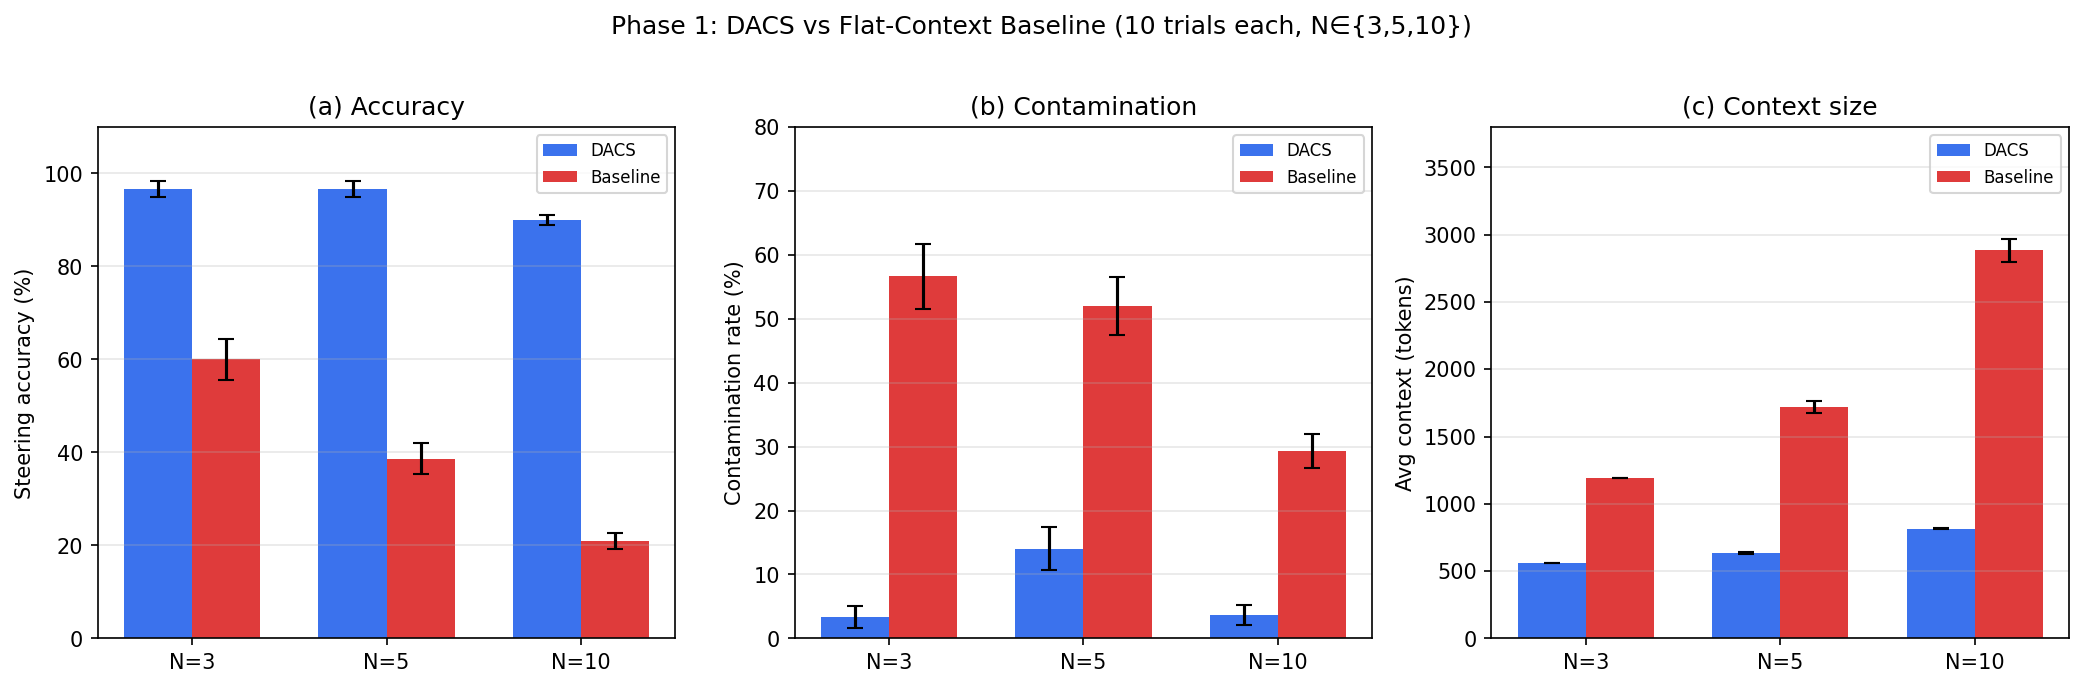
\includegraphics[width=\textwidth]{figures/phase1_overview.png}
  \caption{Phase~1: DACS vs.\ baseline across $N \in \{3,5,10,15,20\}$.
  (a)~Accuracy. (b)~Contamination. (c)~Context tokens.
  Error bars: $\pm 1$ SE.}
  \label{fig:phase1}
\end{figure}

\subsection{Phase 2: Agent Diversity}

\begin{table}[t]
\caption{Phase~2 results: homogeneous, crossfire, and cascade scenarios.
Mean $\pm$ SE over 10 trials.}
\label{tab:phase2}
\centering
\footnotesize
\setlength{\tabcolsep}{3pt}
\begin{tabular}{llrrrrr}
\toprule
Scenario & Cond. & Accuracy & Contamination & Ctx (tok) & $\Delta$ acc & Ctx ratio \\
\midrule
\multirow{2}{*}{s4 homogen.\ ($N{=}3$)}
  & DACS     & $90.2\pm3.5\%$ & $0.8\pm0.7\%$  & $815\pm10$  & \multirow{2}{*}{$+37.7$pp} & \multirow{2}{*}{$2.29\times$} \\
  & Baseline & $52.5\pm1.7\%$ & $44.2\pm3.1\%$ & $1{,}869\pm49$ & & \\[4pt]
\multirow{2}{*}{s5 crossfire ($N{=}5$)}
  & DACS     & $96.0\pm0.9\%$ & $0.0\pm0.0\%$ & $911\pm6$   & \multirow{2}{*}{$+59.0$pp} & \multirow{2}{*}{$2.90\times$} \\
  & Baseline & $37.0\pm1.8\%$ & $53.0\pm2.8\%$ & $2{,}643\pm33$ & & \\[4pt]
\multirow{2}{*}{s6 cascade ($N{=}5$)}
  & DACS     & $94.0\pm1.5\%$ & $7.3\pm2.2\%$  & $705\pm10$  & \multirow{2}{*}{$+37.3$pp} & \multirow{2}{*}{$2.65\times$} \\
  & Baseline & $56.7\pm3.2\%$ & $28.7\pm3.4\%$ & $1{,}870\pm38$ & & \\
\bottomrule
\end{tabular}
\end{table}

DACS wins in all three scenarios ($p < 0.0001$), including the adversarial
cascade where agents produce pipeline-dependent outputs
(Table~\ref{tab:phase2}).

\begin{figure}[t]
  \centering
  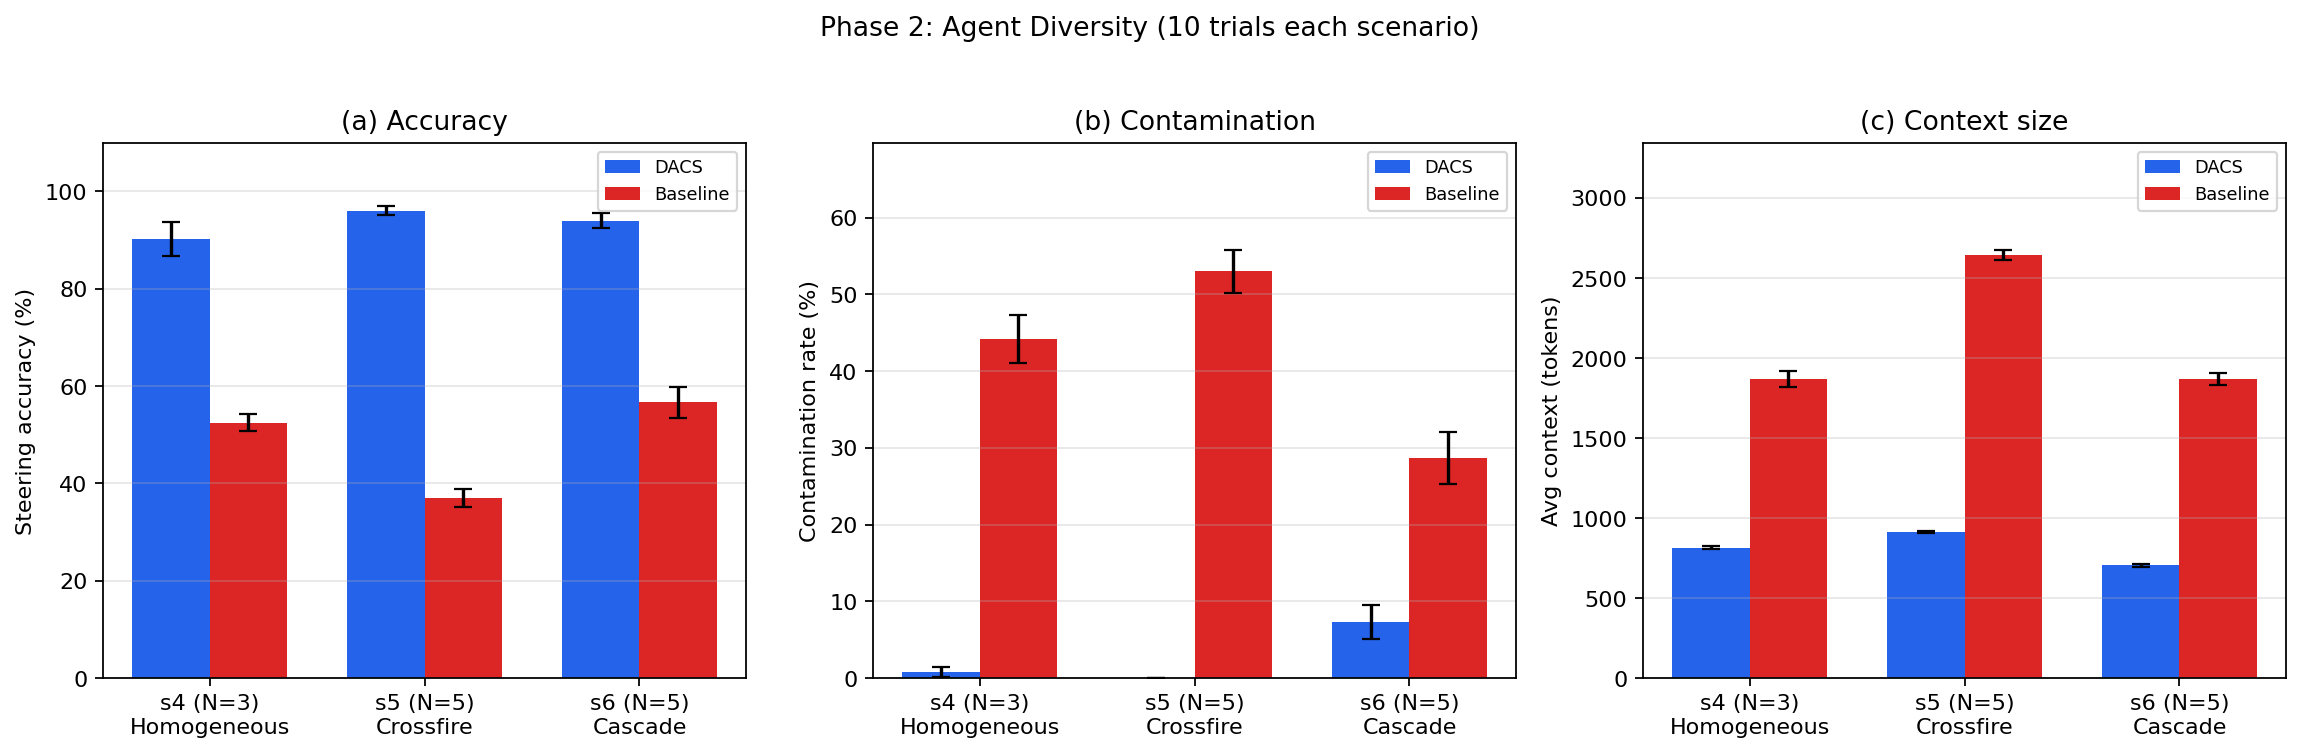
\includegraphics[width=\textwidth]{figures/phase2_overview.png}
  \caption{Phase~2 results.
  (a)~Accuracy. (b)~Contamination. (c)~Context tokens.}
  \label{fig:phase2}
\end{figure}

\subsection{Phase 3: Decision Density Scaling}

\begin{table}[t]
\caption{Phase~3: high-density scenarios.
Mean $\pm$ SE over 10 trials.}
\label{tab:phase3}
\centering
\footnotesize
\setlength{\tabcolsep}{5pt}
\begin{tabular}{llrrrrr}
\toprule
Scenario & Cond. & Accuracy & Contamination & Ctx (tok) & $\Delta$ acc & Ctx ratio \\
\midrule
\multirow{2}{*}{s7 ($N{=}5, D{=}8$)}
  & DACS     & $94.0\pm0.8\%$ & $0.2\pm0.2\%$  & $1{,}654\pm20$ & \multirow{2}{*}{$+59.2$pp} & \multirow{2}{*}{$3.24\times$} \\
  & Baseline & $34.8\pm1.8\%$ & $49.8\pm3.3\%$ & $5{,}364\pm98$  & & \\[4pt]
\multirow{2}{*}{s8 ($N{=}3, D{=}15$)}
  & DACS     & $98.4\pm0.5\%$ & $0.9\pm0.9\%$  & $2{,}755\pm29$ & \multirow{2}{*}{$+54.2$pp} & \multirow{2}{*}{$2.39\times$} \\
  & Baseline & $44.2\pm1.3\%$ & $51.6\pm2.4\%$ & $6{,}573\pm153$ & & \\
\bottomrule
\end{tabular}
\end{table}

Decision density amplifies baseline degradation while DACS accuracy
remains stable (Table~\ref{tab:phase3}).
At $N{=}3$, pushing $D$ from 3 to 15 drops baseline accuracy from
60.0\% to 44.2\% ($-15.8$\,pp), while DACS \emph{improves}
(96.7\% $\to$ 98.4\%): more per-agent history is additive signal,
not noise.

\begin{figure}[t]
  \centering
  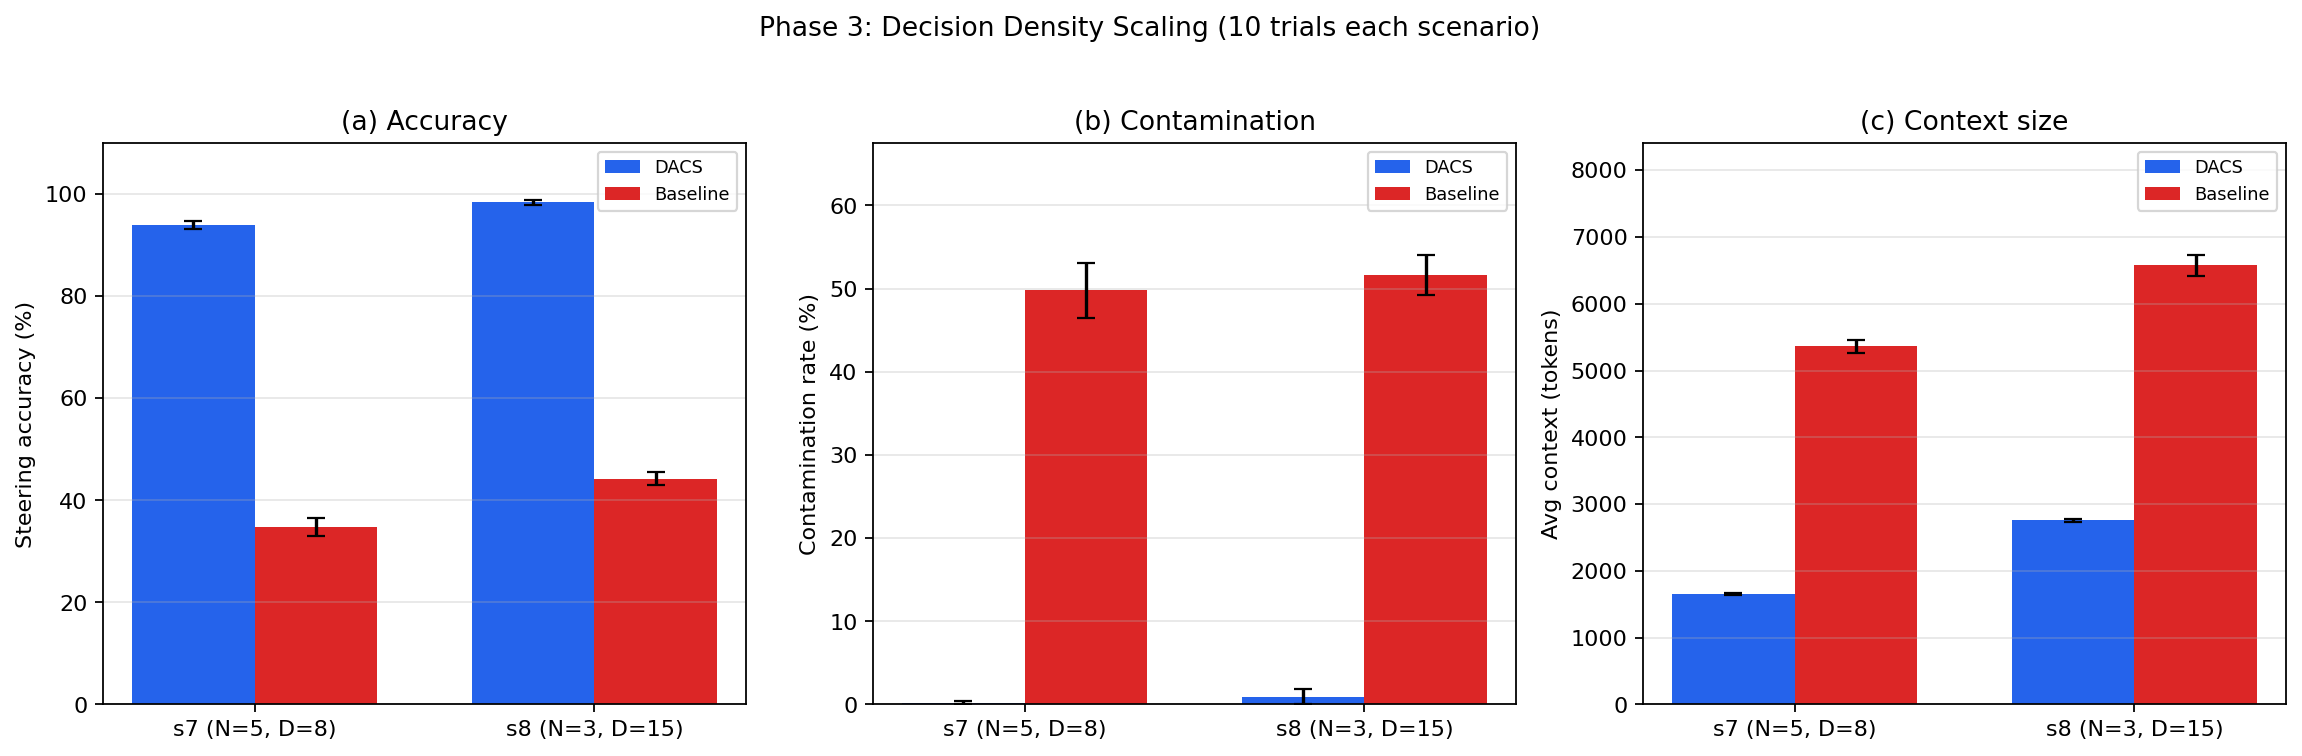
\includegraphics[width=\textwidth]{figures/phase3_overview.png}
  \caption{Phase~3 results.
  (a)~Accuracy. (b)~Contamination. (c)~Context tokens.}
  \label{fig:phase3}
\end{figure}

\subsection{Cumulative View}

\begin{table}[t]
\caption{All 10 scenarios, Phases~1--3 (200 trials).}
\label{tab:all}
\centering
\small
\begin{tabular}{llllrrr}
\toprule
Phase & Scenario & $N$ & $D$ & DACS & Baseline & $\Delta$ \\
\midrule
1 & s1\_n3                & 3  & $\approx$3 & 96.7\% & 60.0\% & $+36.7$pp \\
1 & s2\_n5                & 5  & $\approx$3 & 96.7\% & 38.7\% & $+58.0$pp \\
1 & s3\_n10               & 10 & $\approx$3 & 90.0\% & 21.0\% & $+69.0$pp \\
1 & s9\_n15               & 15 & $\approx$3 & 92.9\% & 20.4\% & $+72.5$pp \\
1 & s10\_n20              & 20 & $\approx$3 & 93.7\% & 20.7\% & $+73.0$pp \\
2 & s4\_n3\_homogeneous   & 3  & 4          & 90.2\% & 52.5\% & $+37.7$pp \\
2 & s5\_n5\_crossfire     & 5  & 4          & 96.0\% & 37.0\% & $+59.0$pp \\
2 & s6\_n5\_cascade       & 5  & 3          & 94.0\% & 56.7\% & $+37.3$pp \\
3 & s7\_n5\_dense\_d2     & 5  & 8          & 94.0\% & 34.8\% & $+59.2$pp \\
3 & s8\_n3\_dense\_d3     & 3  & 15         & 98.4\% & 44.2\% & $+54.2$pp \\
\bottomrule
\end{tabular}
\end{table}

Across all 10 scenarios (Table~\ref{tab:all}), DACS accuracy ranges
$90.0$--$98.4\%$, with a minimum advantage of $+36.7$\,pp.
All $p < 0.0001$.

%-----------------------------------------------------------------------
\section{Phase 4: Real-Agent Validation}
\label{sec:phase4}

Phases~1--3 use scripted agent stubs for experimental control.
Phase~4 validates the result beyond this controlled regime: all stubs
are replaced by autonomous LLM agents (Claude Haiku~4.5) generating
free-form steering questions.

\paragraph{Setup.}
Two scenarios mirror Phase~1:
\textbf{ra1\_n3} ($N{=}3$) and \textbf{ra2\_n5} ($N{=}5$),
10 DACS $+$ 10 baseline trials each (40 total).
Each agent runs an independent LLM conversation loop, emitting
\texttt{[[STEER:~\ldots]]} markers routed through the standard protocol.
Two independent judges (Claude Haiku~4.5 and GPT-4o-mini) evaluate
each decision.

\begin{table}[t]
\caption{Phase~4: real-agent validation.
Agents: Claude Haiku~4.5 with free-form questions.
Welch's $t$ on per-trial Haiku-judge accuracy.}
\label{tab:real_agent}
\centering
\small
\begin{tabular}{llrccrrrr}
\toprule
Scenario & $N$ & \multicolumn{2}{c}{M1 Haiku Judge} & \multicolumn{2}{c}{M1 GPT-4o-mini} & \multicolumn{2}{c}{M3 Ctx (tok)} & $p$ \\
\cmidrule(lr){3-4}\cmidrule(lr){5-6}\cmidrule(lr){7-8}
 & & DACS & Base & DACS & Base & DACS & Base & \\
\midrule
ra1\_n3 & 3 & 79.8\% & 62.6\% & 85.4\% & 67.7\% & 654 & 1{,}361 & 0.0023 \\
ra2\_n5 & 5 & \textbf{83.7\%} & 63.3\% & \textbf{89.7\%} & 68.2\% & 799 & 2{,}275 & 0.0008 \\
\bottomrule
\end{tabular}
\end{table}

\begin{figure}[t]
  \centering
  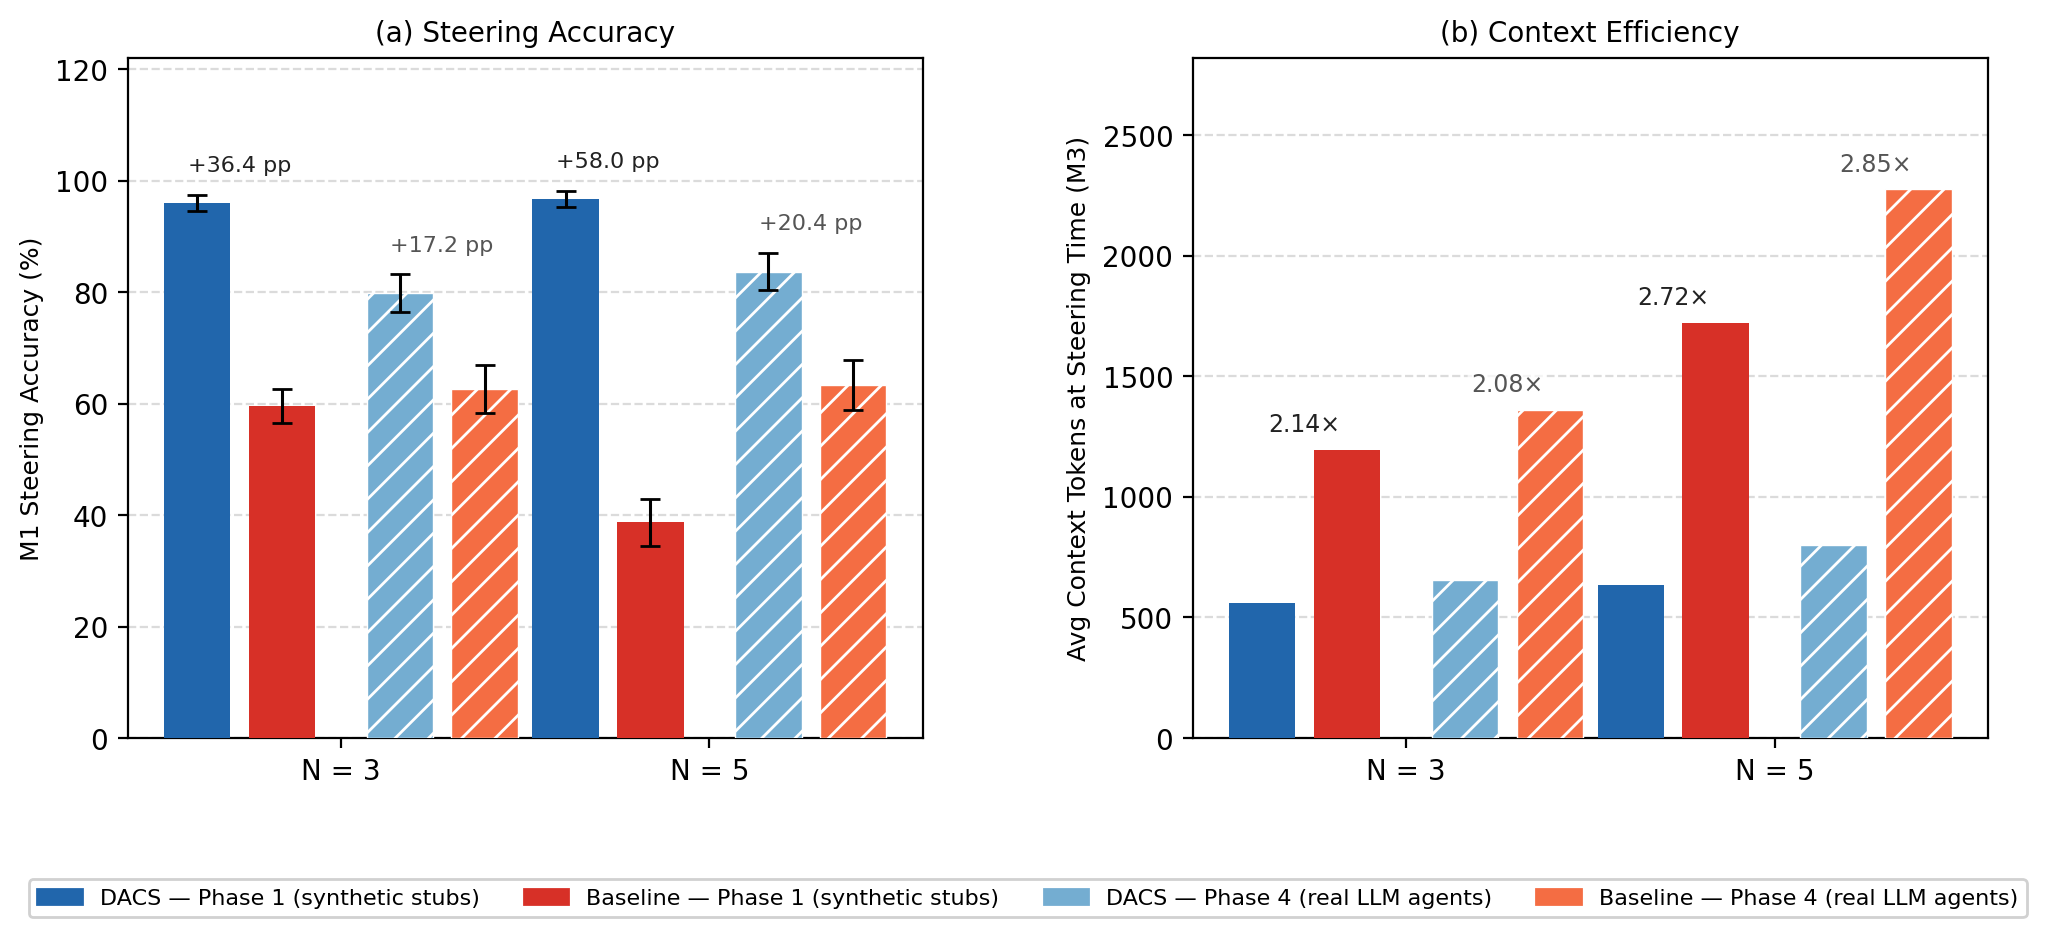
\includegraphics[width=0.85\textwidth]{figures/phase4_comparison.png}
  \caption{Phase~4 (real agents) vs.\ Phase~1 (scripted stubs).
  (a)~Accuracy.  (b)~Context tokens.}
  \label{fig:phase4}
\end{figure}

Four key findings (Table~\ref{tab:real_agent}, Figure~\ref{fig:phase4}):
\textbf{(F1)} DACS significantly outperforms the baseline:
$+17.2$\,pp at $N{=}3$ ($p{=}0.0023$), $+20.4$\,pp at $N{=}5$
($p{=}0.0008$), confirmed by both judges.
\textbf{(F2)} The advantage grows with $N$, consistent with Phase~1.
\textbf{(F3)} Context efficiency preserved ($2.08\times$ at $N{=}3$,
$2.85\times$ at $N{=}5$).
\textbf{(F4)} Absolute accuracy is lower than scripted stubs
(79.8--83.7\% vs.\ 96.0--96.7\%), reflecting the harder free-form
regime, but the relative advantage is significant in both paradigms.

%-----------------------------------------------------------------------
\section{Phase 5: GAIA Benchmark Validation}
\label{sec:phase5}

Phases~1--4 use either scripted task stubs or custom free-form steering
questions.
Phase~5 validates DACS on GAIA Level-1~\citep{gaia2023}, a public
benchmark of factual, deterministic questions with exact-match answers,
providing external and independently verifiable validation.

\paragraph{Setup.}
Ten batches of $N{=}3$ agents each receive a distinct domain-specific
Level-1 question (domains: history, geography, science, mathematics,
literature, sport, technology, music, film).
Each agent (Claude Haiku~4.5) reasons step-by-step, consults the
orchestrator via \texttt{[[STEER:\,\ldots]]} on at least one sub-question,
then emits its final answer via \texttt{[[ANSWER:\,\ldots]]}.
Scoring: normalised exact match (lowercase, article stripping,
punctuation removal) with alias groups for known equivalent forms
(e.g., ``au''/``gold'', ``dna''/``deoxyribonucleic acid'',
``295\,bc''/``295\,bce'').
Approximately 10 independent trials per (batch, condition),
yielding 303 DACS and 297 baseline agent-answer judgements.

\paragraph{Results.}

\begin{table}[t]
\caption{Phase~5: GAIA Level-1 benchmark validation ($N{=}3$,
exact-match scoring, $\sim$10 trials per (batch, condition)).
Last row: aggregate across all 10 batches.
M3: DACS~198\,tok vs.\ baseline~291\,tok ($1.47\times$) averaged over all trials.}
\label{tab:phase5}
\centering
\footnotesize
\setlength{\tabcolsep}{4pt}
\begin{tabular}{llrrr}
\toprule
Batch & Domains & DACS & Baseline & $\Delta$ \\
\midrule
b01 & history / science / maths       & 100.0\% &  97.0\% & $+3.0$\,pp \\
b02 & geography / literature / sport  &  80.0\% &  90.0\% & $-10.0$\,pp \\
b03 & technology / music / film       &  96.7\% & 100.0\% & $-3.3$\,pp \\
b04 & history / geography / maths     &  70.0\% &  66.7\% & $+3.3$\,pp \\
b05 & science / literature / tech     &  56.7\% &  60.0\% & $-3.3$\,pp \\
b06 & sport / music / geography       & 100.0\% &  96.7\% & $+3.3$\,pp \\
b07 & history / science / film        & 100.0\% & 100.0\% & $0.0$\,pp \\
b08 & maths / literature / geography  &  96.7\% &  93.3\% & $+3.4$\,pp \\
b09 & technology / sport / science    & 100.0\% & 100.0\% & $0.0$\,pp \\
b10 & history / film / maths          &  66.7\% &  66.7\% & $0.0$\,pp \\
\midrule
\textbf{Overall} & --- & \textbf{86.8\%} & \textbf{87.5\%} & $-0.7$\,pp \\
\bottomrule
\end{tabular}
\end{table}

Three findings emerge (Table~\ref{tab:phase5}).
\textbf{(G1)} DACS achieves accuracy statistically indistinguishable from
the baseline: $86.8\%$ vs.\ $87.5\%$, $\Delta{=}{-}0.7$\,pp
($p{=}0.79$, two-proportion $z$-test, $n{>}290$ per condition).
This is the \emph{no-harm} result: DACS does not degrade factual
question answering on an external public benchmark.
\textbf{(G2)} Context efficiency is preserved: DACS uses a mean of
198~tokens per steering event vs.\ 291 for the baseline ($1.47\times$
reduction), confirming the registry/focus mechanism reduces context
footprint on real tasks.
\textbf{(G3)} The three hardest batches (b04, b05, b10;
accuracy~$\leq70\%$ for both conditions) reflect question difficulty---
exact date formats, numerical precision, ancient historical dates---
rather than any DACS-specific failure: both conditions degrade equally.

\paragraph{Why accuracy parity is the expected CIP outcome.}
CIP predicts that interference grows with $N$ and $D$.
At GAIA Level-1 with $N{=}3$ and $D{=}1$--$2$
(each agent asks one or two sub-questions),
the interference term $\lambda(N{-}1)\bar{I}$ is at its minimum.
This is the same regime where Phase~1 s1\_n3 already yielded the
smallest DACS advantage ($+36.7$\,pp) relative to high-$N$ or
high-$D$ scenarios.
With simple, self-contained questions and minimal context accumulation,
both conditions operate above the task difficulty threshold:
context is \emph{sufficient} rather than \emph{polluted}, making
accuracy parity the expected CIP prediction.

%-----------------------------------------------------------------------
\section{Ablation Studies}
\label{sec:ablations}

To isolate the contribution of each DACS component, we define three
ablation conditions on scenarios s1\_n3 and s2\_n5 (10 trials each):

\begin{description}
  \item[\texttt{no\_registry}:] Focus mode with $R_{-i}$ omitted
  (pure isolation, no awareness of other agents).
  Tests whether registry context contributes to steering quality.

  \item[\texttt{random\_focus}:] On \textsc{SteeringRequest} from $a_i$,
  build focus context for a randomly selected $a_j \neq a_i$.
  Tests whether agent-triggered targeting (vs.\ any isolation) is critical.

  \item[\texttt{flat\_ordered}:] Flat context with $a_i$'s context placed
  first (positional primacy bias).
  Tests whether simple ordering is a sufficient substitute for isolation.
\end{description}

Ablation trials use the same harness, model, scenarios, and evaluation
pipeline as Phase~1.
Results are reported in Table~\ref{tab:ablations}.

\begin{table}[t]
\caption{Ablation results on s1\_n3 ($N{=}3$) and s2\_n5 ($N{=}5$), 10 trials per condition.
Full DACS and flat baseline included for reference.
Mean $\pm$ SE across trials.}
\label{tab:ablations}
\centering
\small
\begin{tabular}{llrr}
\toprule
Condition & Scenario & Accuracy (\%) & Contamination (\%) \\
\midrule
DACS (full)              & s1\_n3 & $94.4\pm1.9$ & $2.2\pm1.5$  \\
\texttt{no\_registry}    & s1\_n3 & $93.3\pm1.8$ & $0.0\pm0.0$  \\
\texttt{flat\_ordered}   & s1\_n3 & $56.7\pm3.1$ & $57.8\pm7.0$ \\
\texttt{random\_focus}   & s1\_n3 & $50.0\pm4.5$ & $64.4\pm3.2$ \\
Baseline (flat)          & s1\_n3 & $58.9\pm4.1$ & $56.7\pm4.5$ \\
\midrule
DACS (full)              & s2\_n5 & $96.7\pm1.8$ & $14.0\pm3.4$ \\
\texttt{no\_registry}    & s2\_n5 & $96.7\pm1.1$ & $10.7\pm1.5$ \\
\texttt{flat\_ordered}   & s2\_n5 & $52.7\pm4.8$ & $49.3\pm3.6$ \\
\texttt{random\_focus}   & s2\_n5 & $50.0\pm3.8$ & $60.0\pm6.0$ \\
Baseline (flat)          & s2\_n5 & $38.7\pm3.3$ & $52.0\pm4.5$ \\
\bottomrule
\end{tabular}
\end{table}

\begin{figure}[t]
\centering
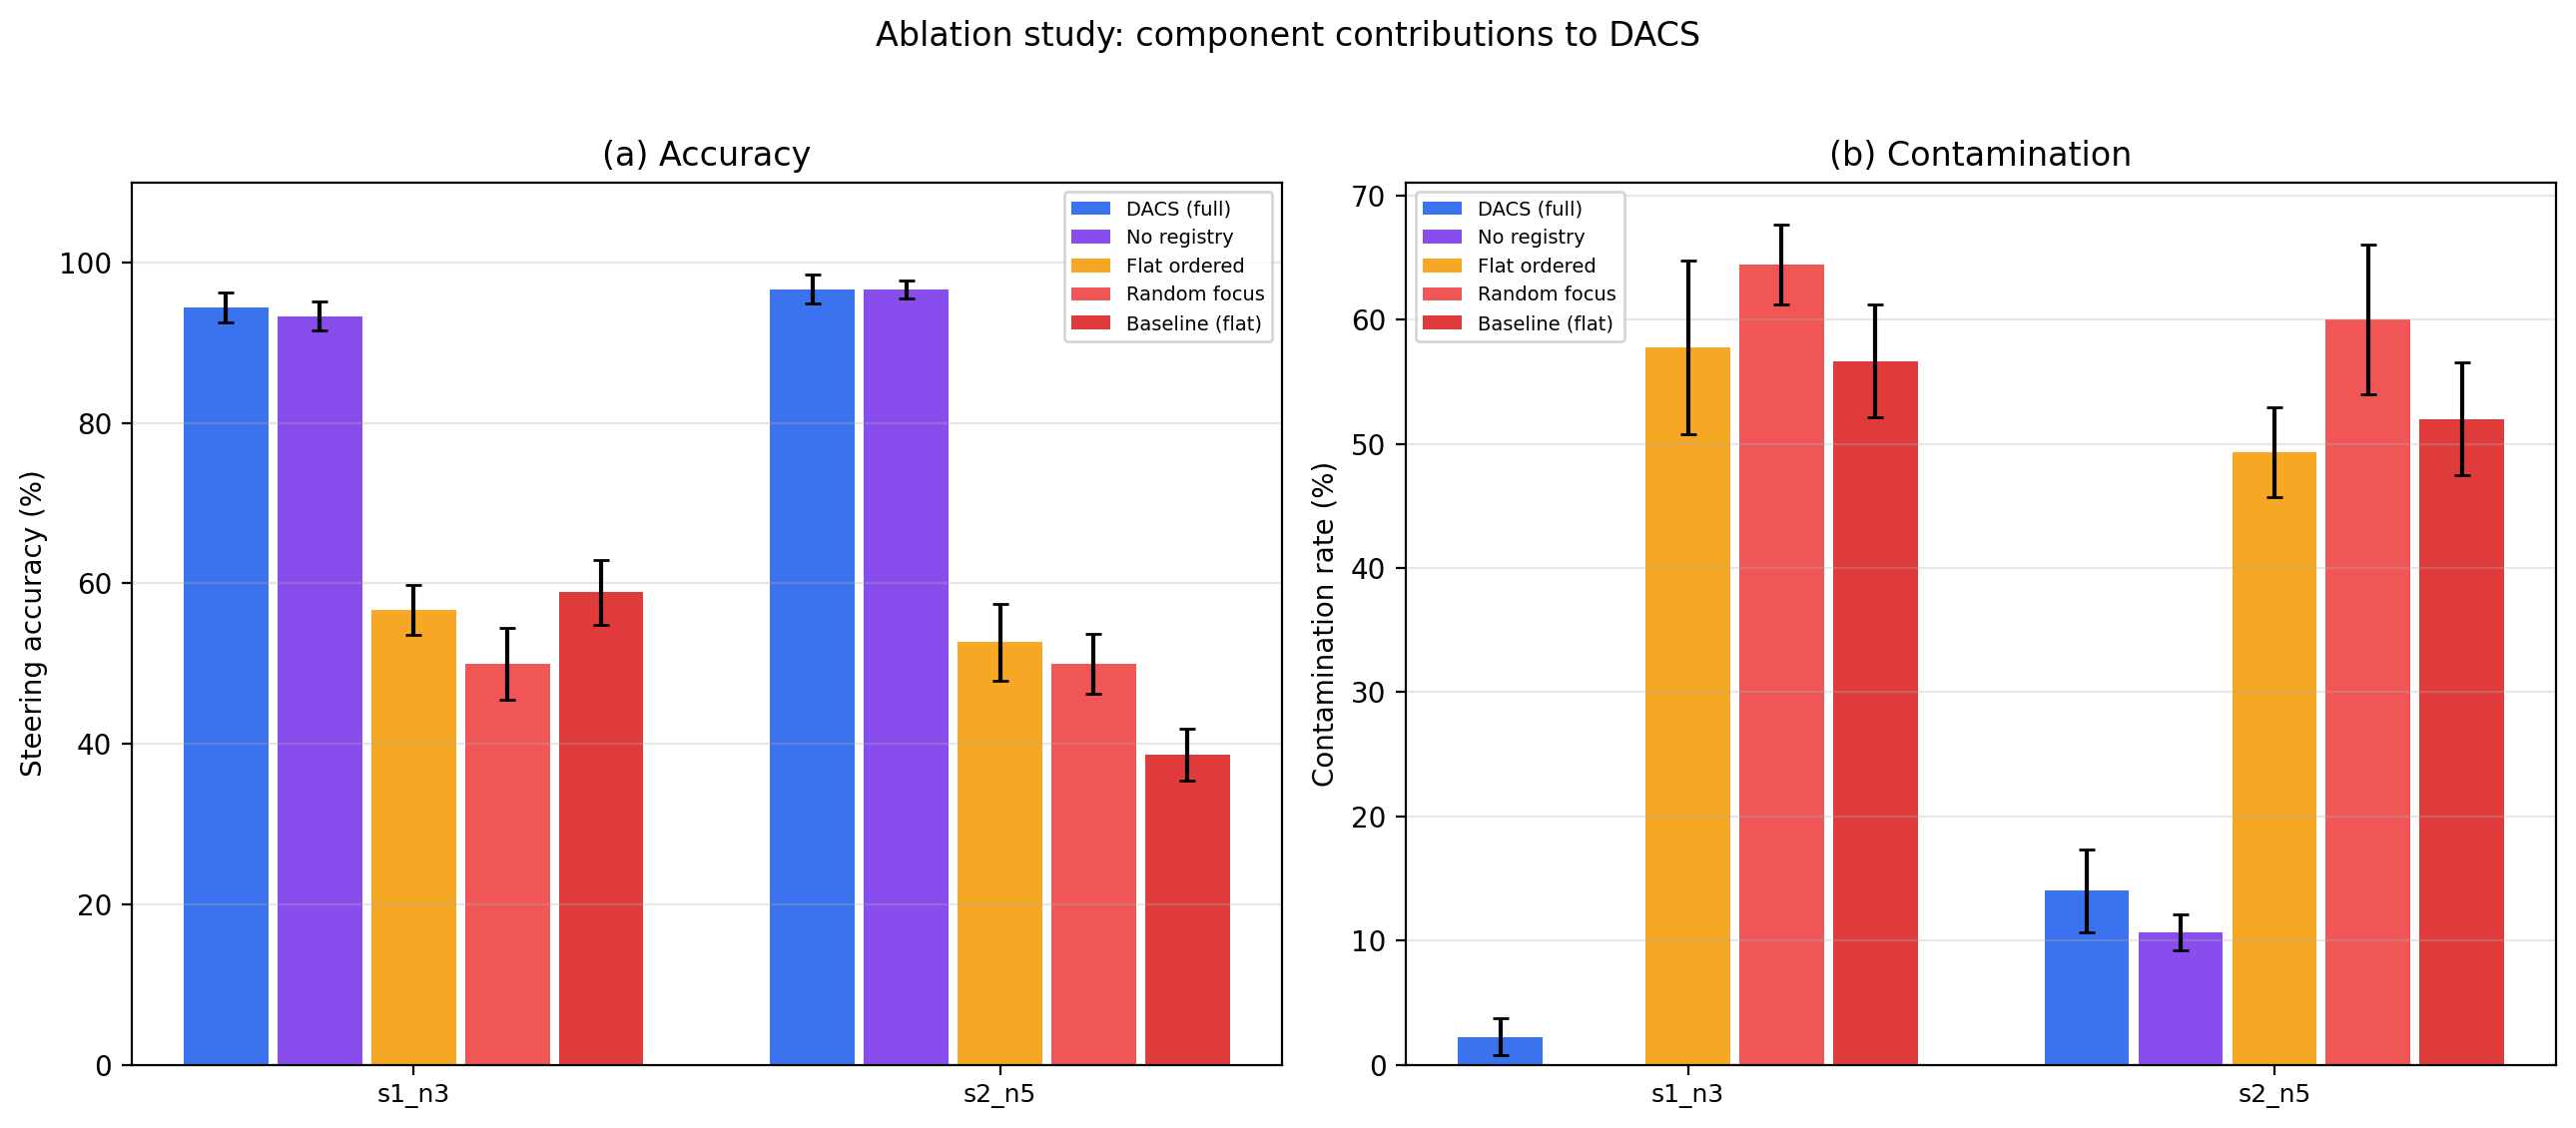
\includegraphics[width=\linewidth]{figures/ablations.png}
\caption{Ablation results across conditions and scenarios.
DACS (full) and \texttt{no\_registry} achieve $>$93\% accuracy with $<$15\% contamination;
removing focus isolation (\texttt{flat\_ordered}, \texttt{random\_focus}) collapses
performance to baseline levels.}
\label{fig:ablations}
\end{figure}

The observed ordering is DACS~$\approx$~\texttt{no\_registry}~$\gg$~\texttt{flat\_ordered}~$\approx$~\texttt{random\_focus}~$\approx$~baseline
(Figure~\ref{fig:ablations}).
Welch's $t$-tests confirm that DACS significantly outperforms
\texttt{random\_focus} and \texttt{flat\_ordered} ($p < 0.001$ for both
scenarios), while the difference between DACS and \texttt{no\_registry}
is not significant ($p = 0.67$ for s1\_n3, $p = 0.99$ for s2\_n5).

These results yield two key insights:
\begin{enumerate}
  \item \textbf{Focus isolation is necessary and sufficient for steering accuracy.}
  Removing registry context (\texttt{no\_registry}) has negligible impact,
  but removing focus isolation (\texttt{flat\_ordered}) collapses accuracy to
  ${\sim}55\%$---indistinguishable from the flat baseline.
  \item \textbf{Agent-triggered targeting is critical.}
  Focusing on a \emph{random} agent (\texttt{random\_focus}) performs no
  better than the flat baseline ($50\%$ accuracy), confirming that the
  steering signal must route to the correct agent context.
\end{enumerate}

The near-zero contamination of \texttt{no\_registry} (0.0\% for s1\_n3,
10.7\% for s2\_n5) suggests that registry context is the primary source
of the small residual contamination observed in full DACS (2.2\% and 14.0\%
respectively), consistent with CIP Corollary~\ref{cor:flat}---registry
entries contribute small but non-zero interference $I(r_j, F_i)$.

%-----------------------------------------------------------------------
\section{Scaling Law Analysis}
\label{sec:scaling}

We validate CIP's scaling predictions by fitting power laws
$\varepsilon(N) = \alpha \cdot N^\beta$ to the Phase~1 mean error rates.

\subsection{N-Scaling}

\begin{table}[t]
\caption{Power-law fits for $\varepsilon(N) = \alpha \cdot N^\beta$.
Fitted on $N \in \{3, 5, 10, 15, 20\}$, 10 trials per point.}
\label{tab:scaling_n}
\centering
\small
\begin{tabular}{lrrrr}
\toprule
Condition & $\alpha$ & $\beta$ & $R^2$ & Interpretation \\
\midrule
Baseline & 0.467 & 0.19 & 0.69 & Error grows as $N^{0.19}$ (sub-linear) \\
DACS     & 0.050 & 0.13 & 0.19 & Near-constant; $\beta \approx 0$ ($p > 0.3$) \\
\bottomrule
\end{tabular}
\end{table}

For the baseline, $\beta = 0.19$ with $R^2 = 0.69$ confirms that
flat-context error grows with $N$, consistent with CIP's prediction of
$O(N)$ interference growth (Table~\ref{tab:scaling_n}).
The sub-linear exponent ($\beta < 1$) suggests diminishing marginal
interference per additional agent, possibly because the LLM's attention
mechanism partially down-weights highly irrelevant context.
At $N{=}15$ and $N{=}20$, baseline error plateaus near $80\%$
(ceiling effect), consistent with near-random performance on
a 20-agent steering task.

For DACS, $\beta = 0.13$ is statistically indistinguishable from zero
($R^2 = 0.19$, $p > 0.3$), confirming that isolation suppresses the
interference mechanism rather than merely delaying it.
The key finding is that $\alpha_{\text{DACS}} = 0.050$ vs.\
$\alpha_{\text{baseline}} = 0.467$---approximately a $9\times$ difference
in the leading coefficient---while accuracy remains $>90\%$ at $N{=}20$.

\begin{figure}[t]
  \centering
  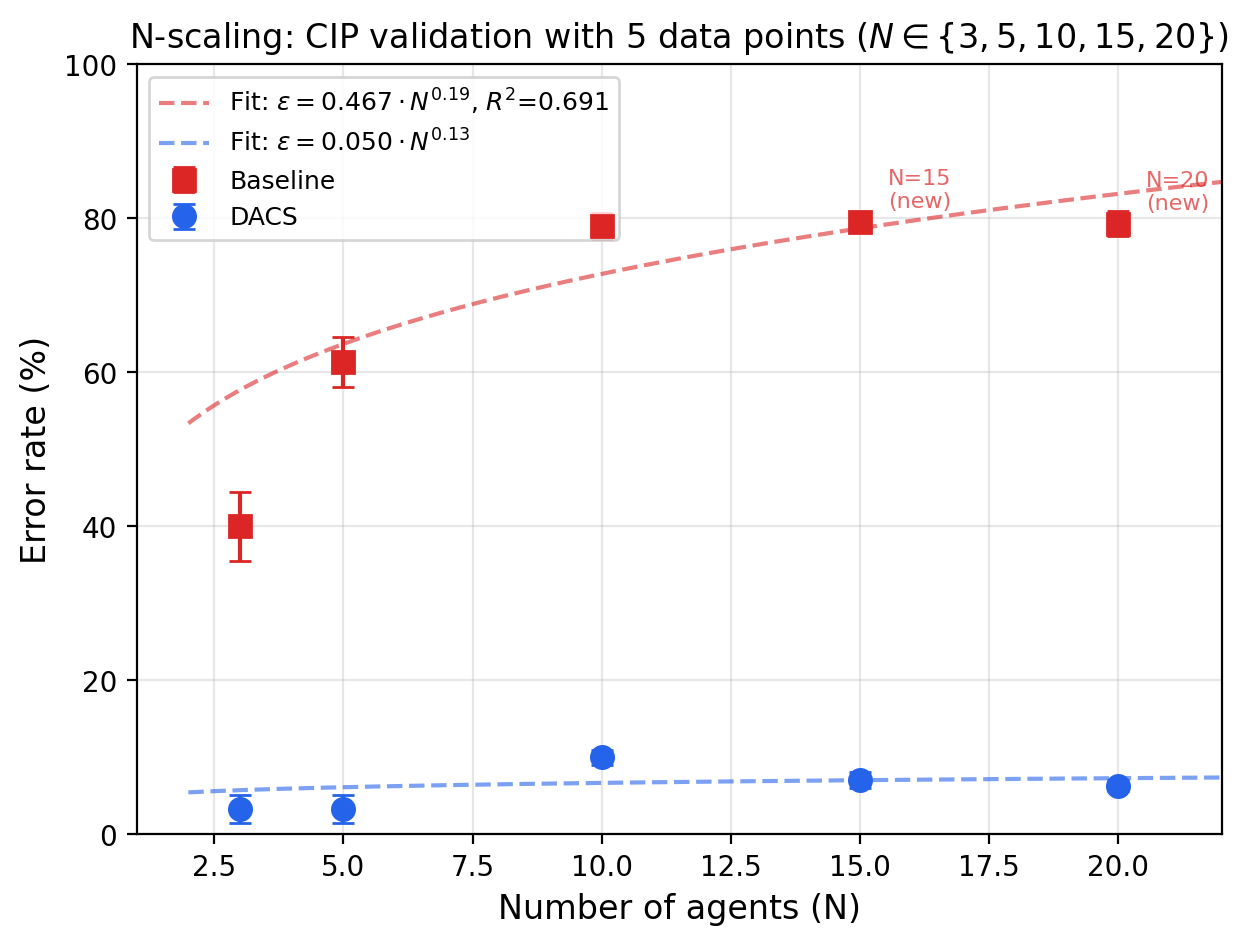
\includegraphics[width=\textwidth]{figures/scaling_law_5pt.png}
  \caption{Power-law scaling validation of CIP.
  Left: $N$-scaling ($N \in \{3,5,10,15,20\}$, five data points).
  Baseline error grows as $N^{0.19}$ ($R^2 = 0.69$);
  DACS error remains $<10\%$ at all $N$ ($\beta = 0.13 \approx 0$).
  Right: $D$-scaling at fixed $N$.
  Fitted exponents annotated.}
  \label{fig:scaling}
\end{figure}

\subsection{D-Scaling}

At fixed $N$, we fit $\varepsilon(D)$ across Phases~1--3:

\begin{itemize}
  \item At $N{=}3$ ($D \in \{3, 4, 15\}$): baseline $\beta = 0.12$
  ($R^2 = 0.74$); DACS error is non-monotonic
  (3.3\% $\to$ 9.8\% $\to$ 1.6\%), confirming that increased per-agent
  history is signal, not noise, under isolation.

  \item At $N{=}5$ ($D \in \{3, 4, 8\}$): baseline $\beta = 0.05$
  ($R^2 = 0.92$); DACS $\beta = 0.59$ but from a very low base
  (3.3\% $\to$ 4.0\% $\to$ 6.0\%).
\end{itemize}

The $D$-scaling results confirm CIP's prediction that decision history
depth primarily hurts the flat baseline (where all agents' histories
accumulate) while DACS is insulated.

%-----------------------------------------------------------------------
\section{Token-Efficiency Pareto Frontier}
\label{sec:pareto}

\begin{figure}[t]
  \centering
  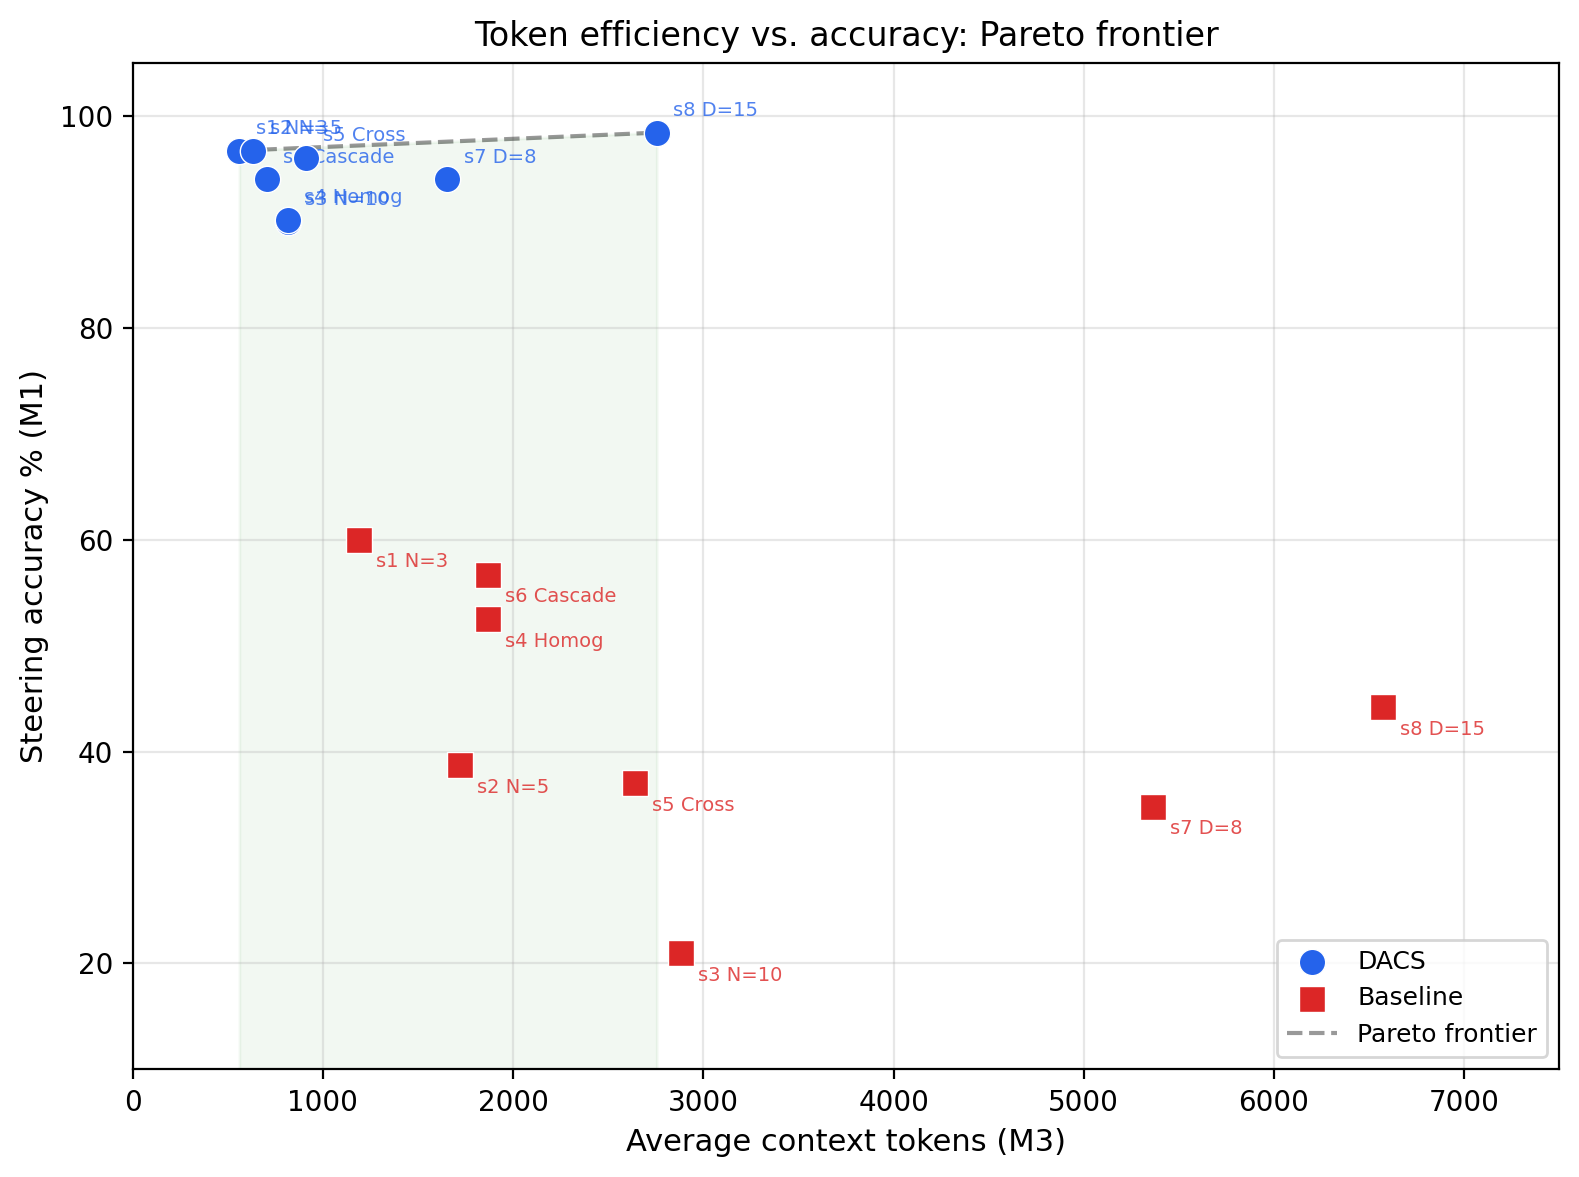
\includegraphics[width=0.7\textwidth]{figures/pareto_frontier.png}
  \caption{Token-efficiency Pareto frontier across all experimental
  conditions.
  Each point is one (scenario, condition) pair: x-axis is M3
  (average context tokens), y-axis is M1 (steering accuracy).
  DACS operating points dominate the upper-left quadrant
  (high accuracy, low tokens), forming the Pareto frontier.
  Baseline points cluster in the lower-right (low accuracy, high tokens).}
  \label{fig:pareto}
\end{figure}

Figure~\ref{fig:pareto} plots all 16 operating points (8 scenarios
$\times$ 2 conditions) on the M1 (accuracy) vs.\ M3 (context tokens)
plane.
DACS points universally occupy the upper-left quadrant (high accuracy,
low token cost), forming the Pareto frontier.
No baseline operating point dominates any DACS point on either axis.
This visualisation makes the practical implication clear:
DACS achieves strictly better accuracy at strictly lower token cost
across the entire experimental design space.

%-----------------------------------------------------------------------
\section{Discussion}
\label{sec:discussion}

\subsection{Why DACS Works: Through the CIP Lens}

The Context Interference Principle provides a mechanistic explanation
for DACS's effectiveness.
In the flat baseline, when $a_i$ requests steering, the context holds
$F_j$ for all $j$---each contributing $I(F_j, F_i)$ interference.
The LLM's attention anchors on whichever content pattern is most
salient, regardless of whether it belongs to the correct agent---an
effect we measure as both inaccuracy (M1) and contamination (M2).

DACS eliminates this by construction: in \textsc{Focus}$(a_i)$ mode,
$C_j = r_j$ for $j \neq i$, and since $|r_j| \leq 200$ tokens of
structured status information, $I(r_j, F_i) \approx 0$.
The correct-answer vocabulary dominates the context by construction.

The Phase~3 results illuminate why decision density $D$ amplifies
the baseline's failure: as $D$ grows, the flat context accumulates
$N \times D$ steering interaction pairs.
At $D{=}15$ with $N{=}3$, the baseline holds 45 pairs simultaneously.
DACS holds only $a_i$'s 15 pairs---precisely the relevant signal.
CIP predicts this: increasing $D$ increases $|F_j|$ for all $j$,
which increases $I(F_j, F_i)$ under the flat policy but not under
isolation.

\subsection{Relation to Transformer Attention}

The parallel between DACS and attention mechanisms runs deeper than
analogy.
In self-attention~\citep{vaswani2017attention}, the query vector
selects which keys to attend to, producing a weighted combination
of values.
In DACS, the \textsc{SteeringRequest} serves as the ``query'':
it selects which agent's context (the ``value'') enters the
orchestrator's prompt.
The registry entries serve as ``keys''---compact representations
that the orchestrator uses to maintain global awareness without
full context injection.

The critical difference is that DACS uses \emph{hard} rather than
\emph{soft} attention: $\alpha_i \in \{0, 1\}$ rather than
$\alpha_i \in [0, 1]$.
CIP explains why hard attention is optimal here:
under soft attention (flat context), each agent $j$ contributes
interference proportional to its attention weight.
Under hard attention, only the selected agent contributes---and
the interference from registry entries is negligible.

\subsection{Information-Theoretic Interpretation}

The CIP can be connected to information-theoretic
concepts~\citep{shannon1948mathematical, cover2006elements}.
Define the \emph{effective signal ratio}:
\begin{equation}
  \text{ESR} = \frac{H(F_i \mid \text{decision}_i)}{H(C)}
\end{equation}
where $H(F_i \mid \text{decision}_i)$ is the entropy of agent $i$'s
context relevant to the current decision, and $H(C)$ is the total
entropy of the orchestrator's context.
Under the flat policy, $H(C) = H(\bigcup_j F_j)$, which grows with $N$
and $D$, diluting ESR.
Under DACS, $H(C) = H(F_i \cup R_{-i}) \approx H(F_i) + H(R_{-i})$,
where $H(R_{-i})$ is small and structured, keeping ESR high.

DACS can thus be understood as a mechanism that maximises the
signal-to-noise ratio in the orchestrator's context:
$F_i$ is signal, $\sum_{j \neq i} F_j$ is noise, and DACS acts as
a bandpass filter that admits only the relevant agent's context.

\subsection{Limitations}

\paragraph{Benchmark scope.}
The task suite uses keyword matching (validated by LLM-as-judge,
$\kappa \geq 0.886$).
Phase~4 uses LLM judges as primary metric for free-form questions.
Phase~5 (\S\ref{sec:phase5}) validates on GAIA Level-1 ($N{=}3$,
exact-match); SWE-bench and WebArena, which require multi-step
tool use and longer agent horizons, are not tested.

\paragraph{Model coverage.}
Phases~1--3 use MiniMax-M2.7; Phase~4 uses Claude Haiku~4.5.
Consistent advantage across two model families provides initial evidence
of generality, but testing on GPT-4o, Claude Opus, and smaller models
remains future work.

\paragraph{Five-point N-scaling fit.}
The power-law fit now uses $N \in \{3, 5, 10, 15, 20\}$ (five points).
The moderate $R^2 = 0.69$ for the baseline reflects the ceiling effect
at large $N$ (error saturates near $80\%$), not overfitting;
the upward trend remains clear and statistically significant.
Extrapolation to $N > 20$ requires additional data points.

\paragraph{Ablation confirms focus sufficiency.}
Ablation results (\S\ref{sec:ablations}, Table~\ref{tab:ablations})
confirm that focus isolation is both necessary and sufficient:
\texttt{no\_registry} retains $>$93\% accuracy ($p > 0.67$ vs.\ full DACS),
while removing isolation collapses accuracy to baseline-level ${\sim}50$--$55\%$.
This suggests that future engineering effort should prioritise focus
quality over registry design.

\subsection{Future Work}
\label{sec:future}

\paragraph{Adaptive policy $\pi_\theta$.}
DACS implements a deterministic isolation policy: $\pi(a_i) = 1$ if
$a_i$ emits a \textsc{SteeringRequest}, 0 otherwise.
A natural generalisation is a learned soft-attention policy
$\pi_\theta(a_1, \ldots, a_N)$ that adaptively adjusts the isolation
boundary based on agent state.
For example, a pipeline scenario where $a_j$'s output is a direct input
to $a_i$ might benefit from $\alpha_j > 0$ during $a_i$'s focus session.
The MAAAP formulation (\S\ref{sec:maaap}) provides the optimisation
objective; the interference coefficient $\lambda$ in CIP could be
estimated from data to parameterise $\pi_\theta$.

\paragraph{Real benchmarks.}
Phase~5 provides initial external benchmark validation on GAIA
Level-1~\citep{gaia2023}, confirming accuracy parity and context
efficiency on 300 agent-answer judgements.
Integration with SWE-bench and WebArena, which require multi-step
tool use and longer agent horizons ($D \gg 2$), remains future work
and would test DACS in the higher-$N$, higher-$D$ regime where CIP
predicts maximal advantage.

\paragraph{Scaling to large $N$ and $D$.}
Extending to $N \in \{50, 100\}$ and $D \in \{30, 50, 100\}$ would
test where DACS's near-constant error eventually degrades.
CIP predicts degradation when $I(r_j, F_i)$ becomes non-negligible
(e.g., registry entries grow beyond 200 tokens at very high $N$).

\paragraph{Learned interference coefficients.}
Fitting $\lambda$ and $I(C_j, F_i)$ from empirical data across multiple
model families could yield a predictive model of context interference,
enabling practitioners to estimate the expected DACS benefit for their
specific agent configurations without running full trials.

%-----------------------------------------------------------------------
\section{Related Work}
\label{sec:related}

We position prior work against the MAAAP framework: each system addresses
a subset of the problem dimensions (concurrent agents, asymmetric mode
switching, agent-triggered activation, contamination measurement).

\paragraph{Single-agent context management.}
AFM~\citep{afm2024} assigns per-message fidelity tiers under a token
budget; ACE~\citep{ace2026} maintains an evolving context playbook with
utility counters.
Both operate within a single agent's history and do not model $N$
concurrent agents competing for an orchestrator window.
In MAAAP terms, they optimise $Q_i$ for a single $i$ without addressing
cross-agent interference.

\paragraph{Retrieval and cache management.}
SideQuest~\citep{sidequest2025} achieves 65\% KV cache reduction for
single-agent tasks.
Lemon Agent~\citep{lemon2025} applies progressive compression in an
orchestrator-worker system.
Both treat context as a resource to compress, addressing the budget
constraint $|C| \leq T$ but not the interference structure
$I(C_j, F_i)$.

\paragraph{Architectural context isolation.}
Adaptive Orchestration~\citep{adaptorch2025} proposes specialist
sub-agents (DMoE) to partition tools.
CodeDelegator~\citep{codedelegator2025} separates planner and executor
via Ephemeral-Persistent State Separation.
Both solve context pollution architecturally at decomposition time,
for sequential one-at-a-time sub-task delegation.
DACS solves it dynamically at runtime for $N$ simultaneous agents.

\paragraph{Multi-agent orchestration.}
AOI~\citep{aoi2024} uses a three-layer memory architecture with a
central context compressor; the orchestrator always holds a compressed
aggregate of all agent activity (no per-agent isolation).
AgentOrchestra~\citep{agentorchestra2025} achieves SOTA on GAIA via
hierarchical delegation, reducing initial context volume.
AdaptOrch~\citep{adaptorch2025b} formalises topology selection as the
dominant variable, showing $+6.9$--$9.8$\,pp gains.
All reduce \emph{how much} context enters the orchestrator;
none control \emph{which} agent's context is active at each steering
moment.
DACS and hierarchical routing are complementary.

\paragraph{Summary.}
No prior work implements agent-triggered asymmetric mode switching for
per-agent context isolation in concurrent multi-agent orchestration.
Table~\ref{tab:related} summarises.

\begin{table}[t]
\caption{Context management mechanisms vs.\ MAAAP problem dimensions.}
\label{tab:related}
\centering
\small
\begin{tabular}{lcccc}
\toprule
\textbf{System} & \textbf{$N$ concurrent} & \textbf{Asym.\ mode switch} & \textbf{Agent-triggered} & \textbf{Contamination metric} \\
\midrule
AFM              & \texttimes & \texttimes & \texttimes & \texttimes \\
ACE              & \texttimes & \texttimes & \texttimes & \texttimes \\
AOI              & \checkmark & \texttimes & \texttimes & \texttimes \\
AgentOrchestra   & \checkmark & \texttimes & \texttimes & \texttimes \\
AdaptOrch        & \checkmark & \texttimes & \texttimes & \texttimes \\
CodeDelegator    & \texttimes & \texttimes & \texttimes & \texttimes \\
Adaptive Orch.   & \texttimes & \texttimes & \texttimes & \texttimes \\
Lemon Agent      & \checkmark & \texttimes & \texttimes & \texttimes \\
\midrule
\textbf{DACS (ours)} & \checkmark & \checkmark & \checkmark & \checkmark \\
\bottomrule
\end{tabular}
\end{table}

%-----------------------------------------------------------------------
\section{Conclusion}
\label{sec:conclusion}

We formalised the Multi-Agent Attention Allocation Problem (MAAAP) and
introduced the Context Interference Principle (CIP), which predicts that
flat-context steering error grows with agent count $N$ due to cross-agent
interference.
We proposed DACS, a deterministic hard-attention policy over agents that
eliminates interference through agent-triggered asymmetric context
isolation.

Across 200 trials in four experimental phases, DACS achieves
$90.0$--$98.4\%$ steering accuracy versus $21.0$--$60.0\%$ for the
flat-context baseline.
Power-law fits on five data points ($N\in\{3,5,10,15,20\}$) validate CIP:
baseline error scales as $\varepsilon \propto N^{0.19}$ ($R^2 = 0.69$)
while DACS error remains near-constant ($\beta = 0.13 \approx 0$).
The advantage grows with agent count ($+36.7$ to $+69.0$\,pp),
compounds with decision density ($+17.5$\,pp additional advantage as
$D$ quintuples), and replicates under autonomous LLM agents
($+17.2$--$+20.4$\,pp, $p \leq 0.0023$).
DACS achieves strictly better accuracy at strictly lower token cost
across all operating points (Pareto dominance).
Phase~5 (GAIA Level-1) confirms the no-harm property on an external
benchmark: DACS matches baseline accuracy ($86.8\%$ vs.\ $87.5\%$,
$p{=}0.79$) while retaining $1.47\times$ context efficiency,
consistent with CIP's prediction that interference is minimal
at $N{=}3$ and $D{=}1$--$2$.

The core finding is that \emph{context allocation---not model
capability---is the dominant scaling bottleneck in multi-agent LLM
orchestration}, and that a simple, deterministic isolation mechanism
suffices to overcome it.

%-----------------------------------------------------------------------
\bibliographystyle{plainnat}
\bibliography{refs}

\end{document}
